\documentclass[11pt,a4paper,openright,twoside]{report}

\usepackage[british]{babel}
\usepackage[utf8]{inputenc}

\usepackage{fancyhdr}
\usepackage{indentfirst}
\usepackage{graphicx}
\usepackage{newlfont}
\usepackage{xcolor}

\usepackage{stmaryrd}
\usepackage{enumitem}


\usepackage{amssymb}
\usepackage{amsmath}
\usepackage{latexsym}
\usepackage{amsthm}
\usepackage{mathabx}

\usepackage{caption}
\usepackage{subcaption}

\usepackage{tikz-cd}

\usepackage[left=2cm,right=2cm,bottom=3cm]{geometry}


\hyphenation{pa-ra-me-tric}
\pagestyle{fancy}\addtolength{\headwidth}{20pt}
\renewcommand{\chaptermark}[1]{\markboth{\thechapter.\ #1}{}}
\renewcommand{\sectionmark}[1]{\markright{\thesection \ #1}{}}
\rhead[\fancyplain{}{\bfseries\leftmark}]{\fancyplain{}{\bfseries\thepage}}
\cfoot{}
\linespread{1}



% Style theorem boxes

\newcounter{mycounter}
\theoremstyle{plain}
\newtheorem{proposition}[mycounter]{Proposition}
\newtheorem{definition}[mycounter]{Definition}
\newtheorem{conjecture}[mycounter]{Conjecture}

\theoremstyle{definition}
\newtheorem{remark}[mycounter]{Remark}
\newtheorem{example}[mycounter]{Example}
\newtheorem{warning}[mycounter]{Warning}


% Quotation marks

\newcommand\dblquote[1]{\textquotedblleft #1\textquotedblright}


%%%%%%%%%%%%%%%%%%%%%%%%% DEDICATION %%%%%%%%%%%%%%%%%%%%%%%%%%%%%%%%%%%%%%%

\begin{document}
\setlist[itemize]{nosep}
\setlist[enumerate]{nosep}

\begin{titlepage}
\thispagestyle{empty}                   
\topmargin=6.5cm                        
\raggedleft                             
\large 
                                 
                                       
\em                                     
To my beloved\\
Benedetta                   
\newpage                                

\clearpage{\pagestyle{empty}\cleardoublepage}
\end{titlepage}
\pagenumbering{roman}


            









































%%%%%%%%%%%%%%%%%%%%%%% INTRODUCTION %%%%%%%%%%%%%%%%%%%%%%%%%%%%%%

\chapter*{Introduction}   
\addcontentsline{toc}{chapter}{Introduction}
\rhead[\fancyplain{}{\bfseries Introduction}]{\fancyplain{}{\bfseries\thepage}}\lhead[\fancyplain{}{\bfseries\thepage}]{\fancyplain{}{\bfseries Introduction}}



\section*{English version}



\section*{Italian version}

\textcolor{blue}{Traduzione italiana dell'introduzione.}


\clearpage{\pagestyle{empty}\cleardoublepage}





















































%%%%%%%%%%%%%%%%%%%%%%%%%%%%% TABLE OF CONTENTS %%%%%%%%%%%%%%%%%%%%%%%%%%%%%%

\tableofcontents
\rhead[\fancyplain{}{\bfseries\leftmark}]{\fancyplain{}{\bfseries\thepage}} \lhead[\fancyplain{}{\bfseries\thepage}]{\fancyplain{}{\bfseries Table of Contents}}
\clearpage{\pagestyle{empty}\cleardoublepage}

























































\chapter{Parametric Optics for Gradient-Based Learning}

\lhead[\fancyplain{}{\bfseries\thepage}]{\fancyplain{}{\bfseries\rightmark}}

\pagenumbering{arabic}



Despite the unquestionable success that gradient-based deep learning has enjoyed in recent years, the field is still both young and poorly understood. As mentioned in the introduction, the lack of theoretical underpinnings means that good performance is highly dependent on \textit{ad hoc} choices and empirical euristics leading to brittleness and poorly understood phenomena (\cite{cruttwell2022categorical}, \cite{shiebler2021category}, \cite{gavranovic2024fundamental}). The ever-growing complexity of deep learning models poses significant challenges both in terms of optimization (\cite{elliott2018simple}) and architectural design (\cite{gavranovicposition}), and, while there are a number of general purpose deep learning libraries that automatically implement backpropagation and provide tools for designing a wide variety of neural networks, these tools often rely on inelegant machinery difficult to parallelize (\cite{elliott2018simple}). Given the ever-increasing role graident based learning plays in the sciences, in industry, and in every day life, solving these issues is of the outmost importance. 

Hence, it would be auspicable to develop a mathematically structured framework for gradient-based learning able to act as a bridge between low-level automatic differentiation and high level architectural specifications (\cite{gavranovic2024fundamental}). The great number of architectures developed in recent years and the inherently modular structure of deep neural networks call for a model which is general (that is, not dependent on a specific differentiation algorithm or a specific optimizer) and compositional (that is, we should be able to predict the behavior of the entire model if the behavior of each part is known). Among the various attempts (see e.g. \cite{fong2019backprop} or \cite{sennesh2023computing}), a promising combination of differential categories, parametrization and optics has been recently proposed by \cite{cockett2019reverse}, \cite{cruttwell2022categorical}, \cite{gavranovic2024fundamental} and more as full-featured gradient-based framework able to challenge established tools. In this chapter, we illustrate such framework  and part of its mathematical foundations. 



\section{Categorical toolkit}

Learning neural networks have two main properties: they depend on parameters and information flows through them bidirectionally (forward propagation and back propagation): any aspiring categorical model of gradient-based learning must take these two aspects into consideration. A number of authors (see e.g. \cite{gavranovic2024fundamental}, and \cite{cruttwell2022categorical}) have proposed the $\mathbf{Para}$ construction as a categorical model of parameter dependence and various categories of optics as the right categorical abstraction for bidirectionality.

\subsection{Actegories}

Before we can deal with parametric maps, we need to find a way to glue input/output spaces to parameter spaces, so that such maps have well-defined domains. One common strategy is to provide the category at hand with a monoidal structure. However, monoidal products can only combine elements within the same underlying category. Since (co)parameters are often taken from spaces that are different in nature from the input and output spaces, a more general mathematical tool is needed: namely, actegories (see the survey \cite{capucci2022actegories} for a thorough treatment of the subject).  Actegories are actions of symmetric monoidal categories on other categories. For brevity's sake, we will only give an incomplete definition (see \cite{capucci2022actegories} or \cite{gavranovic2024fundamental} for further information).

\begin{definition}[Actegory]
  Let $(\mathcal{M},I,\otimes)$ be a strict symmetric monoidal category. A $\mathcal{M}$-actegory is a tuple $(\mathcal{C}, \bullet, \eta, \mu)$, where $\mathcal{C}$ is a category, $\bullet: \mathcal{M} \times \mathcal{C} \to \mathcal{C}$ is a functor, and $\eta$ and $\mu$ are natural isomorphisms enforcing $I \bullet C \stackrel{\eta_C}{\cong}$ and $(M \bullet (N \bullet C)) \stackrel{\mu_{M,N,C}}{\cong} (M \otimes N) \bullet C$.
  The isomorphisms $\eta$ and $\mu$ must also satisfy coherence conditions. If $\eta$ and $\mu$ are identical transformations, we say that the actegory is strict.
\end{definition}

\begin{remark}
  Although the requirement for strictness is somewhat restrictive, we will proceed under the assumption that the actegories we encounter are strict to streamline notation.
\end{remark}

We will also be interested in actegories that interact with the monoidal structure of the underlying category.

\begin{definition}[Monoidal actegory]
  Let $(\mathcal{M},I,\otimes)$ be a strict symmetric monoidal category and let $(\mathcal{C}, \bullet, \eta, \mu)$ be a strict actegory. Suppose $\mathcal{C}$ has a monoidal structure $(J,\boxtimes)$. Then we say that $(\mathcal{C}, \bullet)$ is monoidal if the underlying functor $\bullet$ is monoidal.
\end{definition}


We may also be interested in studying the interaction between actegorical structures and endofunctors. This interaction can happen owing to a natural transformation known as strength. We will not provide coherence diagrams in the definition below for the sake of brevity, but the interested reader can find more detail in \cite{gavranovicposition}. The paper also provides a definition of actegorical strong monad, which is a very similar concept.


\begin{definition}[Actegorical strong functor]
  Let $(\mathcal{C}, \bullet)$ be an $\mathcal{M}$-actegory. A strong actegorical endofunctor on $(\mathcal{C}, \bullet)$ is a pair $(F, \sigma)$ where $F: \mathcal{C} \to \mathcal{C}$ is an endofunctor and $\sigma$ is a natural transformation with components $\sigma_{P,A}: P \bullet F(A) \to F(P \bullet A)$ which satisfies a few coherence conditions that we do not list here.
\end{definition}



\subsection{The $\mathbf{Para}$ construction}


Suppose we have an $\mathcal{M}$-actegory $(\mathcal{C}, \bullet)$. We wish to study maps in $\mathcal{C}$ which are parametrized using objects of $\mathcal{M}$, that is, maps in the form $P \bullet A \to B$. We are not just interested in the maps by themselves, but also in their compositional structure. Thus, we abstract away the details by defining a new category $\mathbf{Para}_{\bullet}(\mathcal{C})$ (first introduced in simplified form in \cite{fong2019backprop}). Since we also want to formalize the role of reparametrization, we actually construct $\mathbf{Para}_{\bullet}(\mathcal{C})$ as a bicategory, so that its $0$-cells $A$ can serve as input/output spaces, its $1$-cells $(P,f)$ can serve as parametric maps, and, finally, its $2$-cells $r$ can serve as reparametrizations.

\begin{definition}[$\mathbf{Para}_{\bullet}(\mathcal{C})$]
  \label{def: para}
  Let $(\mathcal{C}, \bullet)$ be an $\mathcal{M}$-actegory. Then, we define $\mathbf{Para}_{\bullet}(\mathcal{C})$ as the bicategory whose components are as follows.
  \begin{itemize}
    \item The $0$-cells are the objects of $\mathcal{C}$.
    \item The $1$-cells are pairs $(P,f): A \to B$, where $P : \mathcal{C}$ and $f: P \bullet A \to B$.
    \item The $2$-cells come in the form $r: (P,f) \Rightarrow (Q,g)$, where $r: P \to Q$ is a morphism in $\mathcal{C}$. $r$ must also satisfy a naturality condition.
    \item The $1$-cell composition law is
    \[(P,f) \fatsemi (Q,g) = (Q \otimes P, (Q \bullet f)  \fatsemi g).\]
    \item The horizontal and vertical $2$-cell composition laws are respectively given by parallel and sequential composition in $\mathcal{M}$. 
  \end{itemize}
  It is quite handy to represent the cells of $\mathbf{Para}_{\bullet}(\mathcal{C})$ using the string diagram notation illustrated in \textit{Fig. \ref{fig: paramorphisms}}. The $\mathbf{Para}$ construction has a dual $\mathbf{coPara}$ construction whose $1$-cells $f:\mathbf{coPara}_{\bullet}(\mathcal{C})(A,B)$ take the form $(P,f)$, where $f: A \to P \bullet B$. Cells in $\mathbf{coPara}_{\bullet}(\mathcal{C})$ can also be represented with appropriate string diagrams. The reader can find a complete definition in \cite{gavranovic2024fundamental}.
\end{definition}


\begin{figure}[h]
  \begin{center}
    \begin{subfigure}{0.3\textwidth}
      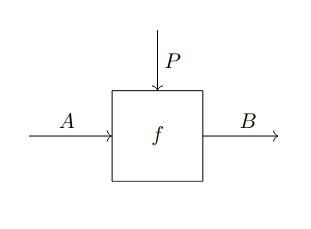
\includegraphics[width=\textwidth]{figures/para.png}
      \caption{}
    \end{subfigure}
    \begin{subfigure}{0.5\textwidth}
      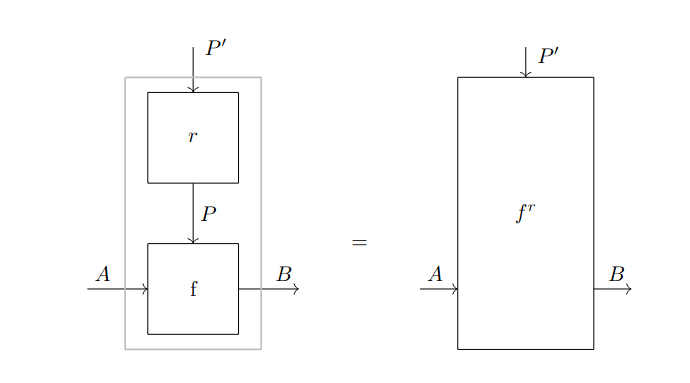
\includegraphics[width=\textwidth]{figures/para_reparametrization.png}
      \caption{}
    \end{subfigure}
    \begin{subfigure}{0.7\textwidth}
      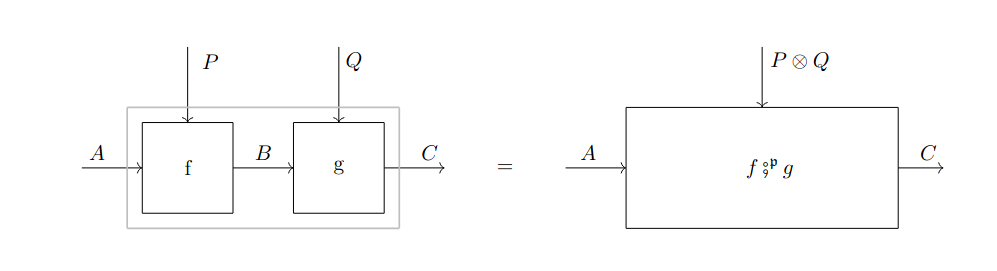
\includegraphics[width=\textwidth]{figures/para_composition.png}
      \caption{}
    \end{subfigure}                 
    \caption[Parametric morphisms]{String diagrams representing (a) a parametric morphism, (b) a reparametrization of a parametric morphism, (c) a composition of parametric morphisms. (Images taken from \cite{gavranovic2024fundamental}.)}\label{fig: paramorphisms}
  \end{center}
\end{figure}


It is shown in \cite{gavranovic2024fundamental} that $\mathbf{Para}_{\bullet}(\mathcal{C})$ is actually a $2$-category if the underlying actegory is strict. Assuming this is the case (as we do in this thesis), we can use a functor $F: \mathbf{Cat} \to \mathbf{Set}$ to quotient out the $2$-categorical structure and turn $\mathbf{Para}_{\bullet}(\mathcal{C})$ into a $1$-category $F_{*}(\mathbf{Para}_{\bullet}(\mathcal{C}))$. Here, $F_{*}: \mathbf{2Cat} \to \mathbf{Set}$ is the change of enrichment basis functor induced by $F$. This meaningfully recovers the $1$-categorical perspective of \cite{fong2019backprop}.


Both $\mathbf{Para}_{\bullet}(\mathcal{C})$ and $\mathbf{coPara}_{\bullet}(\mathcal{C})$ can be given a monoidal structure if $(\mathcal{C}, \bullet)$ is a monoidal actegory. This is extremely important because it allows us to compose (co)parametric morphisms both in sequence and in parallel. Once again, more detail can be found in \cite{gavranovic2024fundamental}.


\begin{remark}
  Another way to parametrize morphisms is the coKleinsli construction. As noted by \cite{gavranovic2024fundamental}, the main difference between $\mathbf{coKl}$ and $\mathbf{Para}$ is that the parametrization offered by $\mathbf{coKl}$ is global, while the parametrization offered by $\mathbf{Para}$ is local: all morphisms in $\mathbf{coKl}(X \times -)$ must take a parameter in $X$, while the parameter space of different morphisms of $\mathbf{Para}(\mathcal{C})$ admit different parameter spaces. Nevertheless, the two constructions are related, and the former can be embedded into the latter.
\end{remark}


If we take a parametrized category $\mathbf{Para}_\bullet(\mathcal{C})$ and we restrict our attention to morphisms parametrized with the monoidal identity $I$, we get back the original category $\mathcal{C}$. This is expressed by the following proposition (\cite{gavranovic2024fundamental}).

\begin{proposition}
  \label{prop: embeddingth}
  Let $(\mathcal{C}, \bullet)$ be an $\mathcal{M}$-actegory. Then, there exists an identity-on-objects pseudofunctor $\gamma: \mathcal{C} \to \mathbf{Para}_\bullet(\mathcal{C})$ that maps $f \mapsto (I,f)$. If $\mathcal{M}$ is strict, this is a $2$-functor.
\end{proposition}




\subsection{Optics}

Modelling bidirectional flows of information is not only useful in machine learning, but also in game theory, database theory, and more. As such, categorical tools for bidirectionality have been sought after for a long time: in particular, the greatest deal of efforts has been devoted to developing lens theory. Lenses have then been generalized into optics (see e.g. \cite{riley2018categories}) to subsume other tools such as prisms and traversals into the same framework. Finally, there have also been various attempts to generalize optics (see e.g. \cite{clarke2024profunctor} for a definition of mixed optics). We will introduce lenses and optics, and focus on the generalization of optics that appears (to us) to be the most versatile: weighted optics (first introduced in \cite{gavranovic2024fundamental}). 


As stated in \cite{gavranovic2024fundamental}, there is no standard definition of lens, and different authors opt for different \textit{ad hoc} definitions that best suit their purposes. We will borrow the perspective of \cite{cruttwell2022categorical} and give the following definition.


\begin{definition}[Lenses]
  \label{def: lenses}
  Let $\mathcal{C}$ be a Cartesian category. Then, $\mathbf{Lens}(\mathcal{C})$ is the category defined by the following data:
  \begin{itemize}
    \item an object of $\mathbf{Lens}(\mathcal{C})$ is a pair $\left(\begin{smallmatrix} A \\ A' \end{smallmatrix}\right)$ of objects in $\mathcal{C}$; 
    
    \item a $\left(\begin{smallmatrix} A \\ A' \end{smallmatrix}\right) \to \left(\begin{smallmatrix} B \\ B' \end{smallmatrix}\right)$ morphism (or lens) is a pair $\left(\begin{smallmatrix} f \\ f' \end{smallmatrix}\right)$ of morphisms of $\mathcal{C}$ such that $f: A \to B$ and $f': A \times B' \to A'$. $f$ is known as the forward pass of the lens $\left(\begin{smallmatrix} f \\ f' \end{smallmatrix}\right)$, whereas $f'$ is known as the bacward pass;
    
    \item given $\left(\begin{smallmatrix} A \\ A' \end{smallmatrix}\right) : \mathbf{Lens}(\mathcal{C})$, the associated identity lens is $\left(\begin{smallmatrix} 1_A \\ \pi_1 \end{smallmatrix}\right)$;
    
    \item the composition of $\left(\begin{smallmatrix} f \\ f' \end{smallmatrix}\right): \left(\begin{smallmatrix} A \\ A' \end{smallmatrix}\right) \to \left(\begin{smallmatrix} B \\ B' \end{smallmatrix}\right)$ and $\left(\begin{smallmatrix} g \\ g' \end{smallmatrix}\right): \left(\begin{smallmatrix} B \\ B' \end{smallmatrix}\right) \to \left(\begin{smallmatrix} C \\ C' \end{smallmatrix}\right)$ is
    \[\left(\begin{smallmatrix} f \fatsemi g \\ \langle \pi_0, \langle \pi_0 \fatsemi f, \pi_1 \rangle \fatsemi g' \rangle \fatsemi f' \end{smallmatrix}\right).\]
  \end{itemize}
  Lenses are best thought of in the helpful language of the string diagrams illustrated in \textit{Fig. \ref{fig: lenses}}.
\end{definition}


\begin{figure}[h]
  \begin{center}
    \begin{subfigure}{0.3\textwidth}
      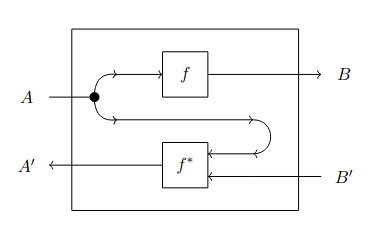
\includegraphics[width=\textwidth]{figures/lens_inner_view.png}
      \caption{}
    \end{subfigure}
    \begin{subfigure}{0.6\textwidth}
      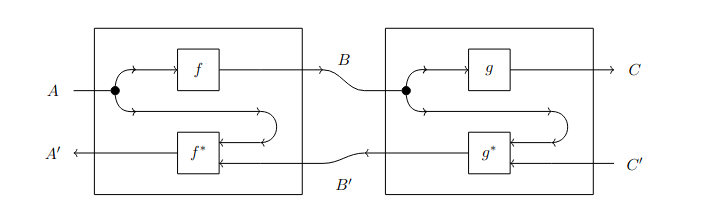
\includegraphics[width=\textwidth]{figures/lens_composition.png}
      \caption{}
    \end{subfigure}                 
    \caption[Lenses]{String diagrams representing (a) a lens $\left(\begin{smallmatrix} f \\ f^* \end{smallmatrix}\right)$, (b) the composition of two lenses $\left(\begin{smallmatrix} f \\ f^* \end{smallmatrix}\right)$ and $\left(\begin{smallmatrix} g \\ g^* \end{smallmatrix}\right)$. (Images taken from \cite{cruttwell2022categorical}.)}
    \label{fig: lenses}
  \end{center}
\end{figure}


Lenses are a powerful tool, but they cannot be used to model all situations: for instance, lenses cannot be used if we wish to be able to choose not to interact with the environment depending on the input, or if we wish like to reuse values computed in the forward pass for further computation in the backward pass.


Optics generalize lenses by weakening the link between forward and bavkward passes, and by replacing the Cartesian structure of the underlying category with a simpler symmetric monoidal structure. In an optic over $\mathcal{C}$, an object $M : \mathcal{C}$ acts as an inaccessible residual space transferring information between the upper components and the lower component.
We will provide the definition given by \cite{riley2018categories}\footnote{\cite{riley2018categories}also provides a more versatile (but more sophisticated) definition of optics that relies on coends. Under the coend formalism,
\[\mathbf{Optic}(\mathcal{C})\left(\left(\begin{smallmatrix} A \\ A' \end{smallmatrix}\right),\left(\begin{smallmatrix} B \\ B' \end{smallmatrix}\right)\right) = \int^{M : \mathcal{C}}\mathcal{C}(A,M \times B) \times \mathcal{C}(M \otimes B',A').\]}, but we will use the string diagram notation presented by \cite{gavranovic2024fundamental} for the sake of consistency.

\begin{definition}[Optics]
  Let $(\mathcal{C}, I, \otimes, \lambda, \rho, \alpha)$ be a symmetric monoidal category (we make the unitors and associators explicit for later use). Then, $\mathbf{Optic}(\mathcal{C})$ is the category defined by the following data:
  \begin{itemize}
    \item an object of $\mathbf{Optic}(\mathcal{C})$ is a pair $\left(\begin{smallmatrix} A \\ A' \end{smallmatrix}\right)$ of objects in $\mathcal{C}$; 
    \item a $\left(\begin{smallmatrix} A \\ A' \end{smallmatrix}\right) \to \left(\begin{smallmatrix} B \\ B' \end{smallmatrix}\right)$ morphism (or optic) is a pair $\left(\begin{smallmatrix} f \\ f' \end{smallmatrix}\right)$ of morphisms of $\mathcal{C}$ such that $f: A \to M \otimes B$ and $f': M \otimes B' \to A'$, where $M : \mathcal{C}$ is known as residual space; such pairs $\left(\begin{smallmatrix} f \\ f' \end{smallmatrix}\right)$ are also quotiented by an equivalence relation that allows for reparametrization of the residual space and effectively makes it inaccessible;
    \item the identity on $\left(\begin{smallmatrix} A \\ A' \end{smallmatrix}\right)$ is the optic represented by $(\lambda_A^{-1}, \lambda_A)$.
  \end{itemize}
  See \cite{riley2018categories} for the more information about how optics compose and about the associated string diagrams.
\end{definition}

Lenses come up as a special case of optics (\cite{riley2018categories}), and optics do solve some of the issues we have with lenses. However, optics are not perfect either: for instance, \cite{gavranovic2024fundamental} points out that optics cannot be used in cases where we ask that the forward pass and backward pass are different kind of maps, as they are both forced to live in the same category. Thus, we need a further layer of generalization: namely, weighted optics.



\subsection{Weighted optics}

Before we define weighted optics, we need to introduce a new tool to our toolbox: the category of elements of a functor.

\begin{definition}[Elements of a functor]
  Let $F: \mathcal{C} \to \mathbf{Set}$ be a functor. We define $\mathbf{El}(F)$ as the category with the following data: (i) the objects of $\mathbf{El}(F)$ are pairs $(C, x)$ where $C : \mathcal{C}$ and $x : F(C)$; (ii) the $(C, x) \to (D, y)$ morphisms in $\mathbf{El}(F)$ are the morphisms $f: C \to D$ in $\mathcal{C}$ such that $F(f)(x) = y$.
\end{definition}

\cite{gavranovic2024fundamental} studies $\mathcal{B}$-actegories $(\mathcal{C}, \bullet)$, which are then reparametrized so that the acting category becomes $\mathcal{E} = \mathbf{El}(W)$ for some weight functor $W: \mathcal{B}^{\mathrm{op}} \to \mathbf{Set}$ (which is to be specified). The reparametrization takes place thanks to the opposite of the forgetful functor $\pi_W: \mathcal{E} \to \mathcal{B}^{\mathrm{op}}$, which maps $(B,x) \mapsto B$. Hence, we consider the action
\[\bullet^{\pi_W^{\mathrm{op}}} = \mathbf{El}(W)^{\mathrm{op}} \times \mathcal{C} \stackrel{\pi_W^{\mathrm{op}} \times \mathcal{C}}{\longrightarrow} \mathcal{B} \times \mathcal{C} \stackrel{\bullet}{\longrightarrow} \mathcal{C}.\]
We are finally ready to define weighted optics\footnote{Weighted optics also admit a coend definition. Refer to \cite{gavranovic2024fundamental} for more information.}.

\begin{definition}[Weighted $\mathbf{coPara}$]
  If $W$ is a weight functor as above and $(\mathcal{C}, \bullet)$ is a $\mathcal{B}$-actegory, we define
  \[\mathbf{coPara}^W_{\bullet}(\mathcal{C}) = \pi_{0*}(\mathbf{coPara}_{\bullet^{\pi_W^{\mathrm{op}}}}(\mathcal{C})),\]
  where $\pi_{0*}$ is the enrichment base change functor generated by the connected component functor $\pi_{0}: \mathbf{Cat} \to \mathbf{Set}$. More explicitly, $\pi_{0*}$ quotients the connections provided by reparametrizations.
\end{definition}

\begin{definition}[Weighted optics]
  Suppose $(\mathcal{C}, \bullet)$ is an $\mathcal{M}$-actegory, suppose $(\mathcal{D}, \sqbullet)$ is an $\mathcal{M}'$-actegory, and suppose $W: \mathcal{M}^{\mathrm{op}} \times \mathcal{M}' \to \mathbf{Set}$ is a lax monoidal functor.
  We define the category of $W$-weighted optics over the product actegory $\left(\mathcal{C}\times\mathcal{D}^{\mathrm{op}},\left(\begin{smallmatrix}\bullet\\\sqbullet^{\mathrm{op}}\end{smallmatrix}\right)\right)$ as
  \[\mathbf{Optic}^W_{\left(\begin{smallmatrix}\bullet\\\sqbullet\end{smallmatrix}\right)} = \mathbf{coPara}^W_{\left(\begin{smallmatrix}\bullet\\\sqbullet^{\mathrm{op}}\end{smallmatrix}\right)}(\mathcal{C}\times\mathcal{D}^{\mathrm{op}}).\]
\end{definition}

The definition is very dense and deserves some explanation. Fist of all, we assume that $W$ maps $(M,M')$ to a set of maps $s: M \to M'$. If that's the case, a $\left(\begin{smallmatrix}X\\X'\end{smallmatrix}\right) \to \left(\begin{smallmatrix}Y\\Y'\end{smallmatrix}\right)$ map is a triplet $\left(\left(\begin{smallmatrix}\\M'\end{smallmatrix}\right),s,\left(\begin{smallmatrix}f\\f'\end{smallmatrix}\right)\right)$, where $M$ is the forward residual, $M'$ is the backward residual, $s: M \to M'$ links the two residuals, $f: X \to M \bullet Y$ is the forward pass, and $f': M' \bullet Y' \to X'$ is the backward pass.
The triplets are also quotiented with respect to reparametrization, which makes the residual spaces effectively inaccessible (as it happens in the case of ordinary optics). We can get a clear "operational" understanding of how a weighted optic works looking at an associated string diagram: data from $X$ flows through the forward map, which computes an output in $Y$ and a forward residual in $M$. Such forward residual is then converted into a backward residual in $M'$ by the map $s$, which is provided by the weight functor. Finally, the backward residual is used to compute, together with input from $Y'$ a value in $X'$. The last step happens thanks to the backward map $f'$. A full account of the composition law for weighted optics can be found on \cite{gavranovic2024fundamental}.
As stated in \cite{gavranovic2024fundamental}, since $\mathbf{coPara}$ can be given a monoidal structure, we can also give $\mathbf{Optic}^W_{\left(\begin{smallmatrix}\bullet\\\sqbullet\end{smallmatrix}\right)}$ one such structure as long as the underlying actegories are monoidal and the weight functor $W$ is braided monoidal.


The advantages of weighted optics over ordinary optics are clear: when dealing with weighted optics, we are no longer forced to take reverse maps from the same category as the forward maps. The action on the category of forward spaces is now separated from the action on the category of backward spaces, and the link between the two actions is provided by an external functor. Such modular approach provides a great deal of conceptual clarity and flexibility, more than regular optics or lenses can provide on their own. It is also shown in \cite{gavranovic2024fundamental} that weighted optics are indeed a generalization of optics. In particular, it is shown that the lenses in \textit{Def. \ref{def: lenses}} are the specialized weighted optics obtained when $\mathcal{C} = \mathcal{D}$ is Cartesian and the actegories are given by the Cartesian product. More generally, \cite{gavranovic2024fundamental} claims that - to the best of the author's knowledge - all definitions of lenses currently used in the literature are subsumed by the definition of weighted optics.


\cite{gavranovic2024fundamental} goes on to apply the $\mathbf{Para}$ construction onto weighted optics, obtaining parametric weighted optics, which are proposed as a full-featured model for deep learning. The author conjectures that "weighted optics provide a good denotational and operational semantics for differentiation". In its full, generality, this is still an unproven conjecture. However, restricting our attention to a special class $\mathbf{Lens}_A$ of lenses with an additive backward passes yields a fully formal theory of structural backpropagation, which will be illustrated in the rest of the capter, after a short digression on differential categories.





\subsection{Differential categories}
\label{subsec: diffcats}


Modelling gradient-based learning obviously requires a setting where differentiation can take place. Although it is tempting to directly employ smooth functions over Euclidean spaces, recent research has shown that there are tangible advantages in working with generalized differential combinators that extend the notion of derivative to polynomial circuits (\cite{wilson2022categories}, \cite{wilson2021reverse}), manifolds (\cite{peng2021hyperbolic}), complex spaces (\cite{bassey2021survey}), and so on.  Thus, it makes sense to work with an abstract notion of derivative which can then be appropriately implemented depending on the requirements at hand.


One approach to this problem involves the explicit definition of two kidns of differential categories: Cartesian differential categories (first introduced in \cite{blute2006differential}) and Cartesian reverse differential categories (first introduced by \cite{cockett2019reverse}). The former allow for forward differentiation, while the latter allow for reverse differentiation. We will omit the defining axioms for the sake of brevity, but the reader can find complete definitions in \cite{cockett2019reverse}.

\begin{definition}[Cartesian differential category]
  \label{def: cdc}
  A Cartesian differential category (CDC) $\mathcal{C}$ is a Cartesian left-additive category where a differential combinator $\mathrm{D}$ is defined. Such differential combinator must take a morphism $f: A \to B$ and return a morphism $\mathrm{D}[f]: A \times A \to B$, which is known as the derivative of $f$. The combinator $\mathrm{D}$ must satisfy a number of axioms. 
\end{definition}

\begin{definition}[Cartesian reverse differential category]
  A Cartesian reverse differential category (CRDC) $\mathcal{C}$ is a Cartesian left-additive category where a reverse differential combinator $\mathrm{R}$ is defined. Such reverse differential combinator must take a morphism $f: A \to B$ and return a morphism $\mathrm{R}[f]: A \times B \to A$, which is known as the reverse derivative of $f$. The combinator $\mathrm{R}$ must satisfy a number of axioms. 
\end{definition}

\begin{example}
  \label{ex: smooth}
  $\mathbf{Smooth}$ is a both a CDC and a CRDC. In fact, if $\mathcal{J}_f$ is the Jacobian matrix of a smooth morphism $f$,
  \[\mathrm{D}[f]: (x,v) \mapsto \mathcal{J}_f(x)v\]
  and
  \[\mathrm{R}[f]: (x,y) \mapsto \mathcal{J}_f(x)^Ty\]
  induce well-defined combinators $\mathrm{D}$ and $\mathrm{R}$. This is only a partial coincidence, as shown in \cite{cockett2019reverse} that CRDCs are always CDCs under a canonical choice of differential combinator. The converse, however, is generally false.
\end{example}


As it turns out, forward differentiation tends to be less efficient when dealing with neural networks that come up in practice (\cite{elliott2018simple}), so CDCs are not extremely useful when studying deep learning. CRDCs, on the other hand, have been applied to great success (see e.g. \cite{cruttwell2022categorical}). As shown in \cite{wilson2022categories}, a large supply of CRDCs can be obtained by providing the generators of a finitely presented Cartesian left-additive category with associated reverse derivatives (as long as the choices of reverse derivative are consistent).
Moreover, CRDCs have been recently generalized by \cite{gavranovic2024fundamental} to coalgebras associated with copointed endofunctors, which could also increase the number of known CRDCs in the future. The rest if this section is devoted to this generalization.


It is shown in \cite{gavranovic2024fundamental} that there is a particular class of weighted optics which is useful for reverse differentiation, being able to represent both maps (through forward passes) and the associated reverse derivatives (through backward passes). Moreover, such weighted optics can be represented as lenses in the sense of \textit{Def \ref{def: lenses}}, which means that their inner workings can be pictured in a simple, intuitive way.


\begin{definition}[Additively closed Cartesian left-additive category]
  A Cartesian left-additive category $\mathcal{C}$ is an additively closed Cartesian left-additive category (ACCLAC) if and only if the following are true:
  \begin{itemize}
    \item the subcategory $\mathbf{CMon}(\mathcal{C})$ of additive maps has a closed monoidal structure $(I, \otimes)$;
    \item the embedding $\iota: \mathbf{CMon}(\mathcal{C}) \to \mathcal{C}$ is a lax monoidal funtor with respect to the aforementioned structure of $\mathbf{CMon}(\mathcal{C})$ and the Cartesian structure of $\mathcal{C}$.
  \end{itemize}
\end{definition}


Then, we can define the category of lenses with backward passes additive in the second component.

\begin{definition}
  Let $\mathcal{C}$ be an ACCLAC with Cartesian structure is $(1, \times)$ and whose subcategory $\mathbf{CMon}(\mathcal{C})$ has monoidal structure $(I, \otimes)$. Then, we define
  \[\mathbf{Lens}_A(\mathcal{C}) = \mathbf{Optic}_{\left(\begin{smallmatrix}\times \\ \otimes\end{smallmatrix}\right)}^{\mathcal{C}(-,\iota(-))}.\]
\end{definition}

As argued in \cite{gavranovic2024fundamental}, the symbol $\mathbf{Lens}_A$ is justified because one such optic of type $\left(\begin{smallmatrix}X \\ X'\end{smallmatrix}\right) \to \left(\begin{smallmatrix}Y \\ Y'\end{smallmatrix}\right)$ can be concretely represented as a lens with forward pass $f : \mathcal{C}(X,Y)$ and backward pass $f' : \mathcal{C}(X \times Y',X')$, which is the approach we illustrate in this thesis.  Nevertheless, some potential expressiveness is lost when passing from weighted optic composition to concrete lens composition. In particular, if we operated with optics, we would be able to implement backpropagation without resorting to gradient checkpointing, which is not possible if we use lenses (\cite{gavranovic2024fundamental}). 


The generalization mentioned above is possible because $\mathbf{Lens}_A$ is an endofunctor.

\begin{definition}
  We defined $\mathbf{CLACat}$ as the category whose objects are Cartesian left-additive categories and whose morphisms are Cartesian left-additive functors (see e.g.\cite{blute2006differential}).
\end{definition}

\begin{proposition}
  If $\mathcal{C} : \mathbf{CLACat}$, then $\mathbf{Lens}_A(\mathcal{C}) : \mathbf{CLACat}$.
\end{proposition}
\begin{proof}
  The Cartesian structure on $\mathbf{Lens}_A(\mathcal{C})$ is given by $\left(\begin{smallmatrix}X \\ X'\end{smallmatrix}\right) \times \left(\begin{smallmatrix}Y \\ Y'\end{smallmatrix}\right) = \left(\begin{smallmatrix}X\times Y \\ X' \times Y'\end{smallmatrix}\right)$ and by the initial object $\left(\begin{smallmatrix}1 \\ 1\end{smallmatrix}\right)$. The monoidal structure on each $\left(\begin{smallmatrix}X \\ X'\end{smallmatrix}\right)$ is given by the unit $0_{\left(\begin{smallmatrix}X \\ X'\end{smallmatrix}\right)} = \left(\begin{smallmatrix}0_A \\ !_{1 \times A'}\end{smallmatrix}\right): \left(\begin{smallmatrix}1 \\ 1\end{smallmatrix}\right) \to \left(\begin{smallmatrix}X \\ X'\end{smallmatrix}\right)$ and by the multiplication $+_{\left(\begin{smallmatrix}X \\ X'\end{smallmatrix}\right)} = \left(\begin{smallmatrix}+_A \\ \pi_2 \fatsemi \Delta_{A'}\end{smallmatrix}\right): \left(\begin{smallmatrix}X \times X \\ X' \times X'\end{smallmatrix}\right) \to \left(\begin{smallmatrix}X \\ X'\end{smallmatrix}\right)$.
\end{proof}

\begin{proposition}
  $\mathbf{Lens}_A: \mathbf{CLACat} \to \mathbf{CLACat}$ is a functor.
\end{proposition}
\begin{proof}
  Given a Cartesian left-additive functor $F: \mathcal{C} \to \mathcal{D}$, we can define $\mathbf{Lens}_A(F)$ as the functor that maps $\left(\begin{smallmatrix}X  \\ X' \end{smallmatrix}\right) \mapsto \left(\begin{smallmatrix} F(X) \\ F(X') \end{smallmatrix}\right)$ and maps $\left(\begin{smallmatrix}f  \\ f' \end{smallmatrix}\right) \mapsto \left(\begin{smallmatrix} F(f) \\ \underline{f} \end{smallmatrix}\right)$, where $\underline{f} = F(X) \times F(Y')) \stackrel{\cong}{\longrightarrow} F(X \times Y') \stackrel{F(f')}{\longrightarrow}F(X')$. It can be shown that $\mathbf{Lens}_A(F)$ is also Cartesian left-additive.
\end{proof}

\begin{proposition}
  $\mathbf{Lens}_A$ has a copointed structure\footnote{An endofunctor $F: \mathcal{C} \to \mathcal{C}$ is copointed if it is endowed with a natural transformation $\epsilon: F(\mathcal{C}) \Rightarrow \mathrm{id}_{\mathcal{C}}$.}.
\end{proposition}
\begin{proof}
  It suffices to endow $\mathbf{Lens}_A$ with the natural transformation $\epsilon$ whose components are the forgetful functors $\epsilon_{\mathcal{C}}: \mathbf{Lens}_A(\mathcal{C}) \to \mathcal{C}$ which strip away the backward passes.
\end{proof}

Hence, \cite{gavranovic2024fundamental} defines generalized CRDCs as follows.

\begin{definition}[Generalized Cartesian reverse differential category]
  A generalized Cartesian reverse differential category is a coalgebra for the pointed endofunctor $\mathbf{Lens}_A$. 
\end{definition}

Explicitly, a colagebra for $\mathbf{Lens}_A$ is a pair $(\mathcal{C}, \mathbf{R}_{\mathcal{C}})$ such that $\mathcal{C}: \mathbf{CLACat}$ and $\mathbf{R}_{\mathcal{C}}: \mathcal{C} \to \mathbf{Lens}_A(\mathcal{C})$ satisfies $\mathbf{R}_{\mathcal{C}} \fatsemi \epsilon_{\mathcal{C}} = \mathrm{id}_{\mathcal{C}}$. The intuition behind such definition is that $\mathbf{R}_{\mathcal{C}}$ should map $f \mapsto \left(\begin{smallmatrix} f \\ R[f] \end{smallmatrix}\right)$, where $R[f]$ is a generalized reverse derivative combinator. \cite{gavranovic2024fundamental} shows that such a definition of $\mathbf{R}_{\mathcal{C}}$ does indeed prove that ordinary CRDC fall into the definition of generalized CRDC. 


\subsection{Parametric lenses}

We conclude this section discussing the relation between the $\mathbf{Para}$ construction and the $\mathbf{Lens}_A$ endofunctions. \cite{gavranovic2024fundamental} shows that, under an appropriate definition, \lq morphisms of actegories induce morphisms of parametric bicategories\rq. As a consequence, it can be shown that, if  $(\mathcal{C}, \mathbf{R}_{\mathcal{C}})$ is a generalized CRDC,  $\mathbf{R}_{\mathcal{C}}$ induces a functor $\mathbf{Para}(\mathbf{R}_{\mathcal{C}}): \mathbf{Para}_{\times}(\mathcal{C}) \to \mathbf{Para}_{\bullet}(\mathbf{Lens}_A(\mathcal{C}))$, which takes a parametric map $f: P \times A \to B$ and augments is with its reverse derivative $\mathrm{R}[f]$, forming a parametric lens. Parametric lenses behave very similarly to lenses, but we provide a separate stand-alone definition (which we take from \cite{cruttwell2022categorical}) for the reader's convenience.

\begin{definition}[Parametric lenses]
  The category of parametric lenses over a Cartesian category $(\mathcal{C},1,\times)$ is $\mathbf{Para}_{\bullet}(\mathbf{Lens}(\mathcal{C}))$, where $\bullet$ is the action on the lenses generated by the Cartesian structure of $\mathcal{C}$:
  \[\begin{pmatrix}
    P \\ P'
  \end{pmatrix} \bullet \begin{pmatrix}
    A \\ A'
  \end{pmatrix} = \begin{pmatrix}
    P \times A \\ P' \times A'
  \end{pmatrix}.\]
  Refer to \textit{Fig. \ref{fig: paralenses}} to see a string diagram that shows the inner workings of a parametric lens.
\end{definition}

\begin{figure}[h]
  \begin{center}
    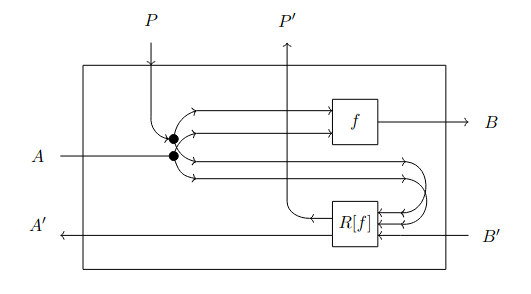
\includegraphics[width=0.5\textwidth]{figures/parametric_lens.png}             
    \caption[Parametric lens]{String diagrams representing the inner workings of a parametric lens. (Images taken from \cite{cruttwell2022categorical}.)}
    \label{fig: paralenses}
  \end{center}
\end{figure}





\section{Supervised learning with parametric lenses}
\label{sec: opticbasedlearning}

In this section, we show how parametric lenses can be used to model supervised gradient-based learning (\cite{cruttwell2022categorical}, \cite{gavranovic2024fundamental}, \cite{shiebler2021category}). While lenses are not as general as weighted optics, it is shown in \cite{cruttwell2022categorical} that they are powerful enough for most purposes and that there is some empirical evidence of their performance and applicability. The paper also discusses the use of parametric lenses in modeling unsupervised deep learning and deep dreaming, but we do not have the space to discuss them here.

\subsection{Model, loss, optimizer, learning rate}

Supervised gradient-based learning can be modeled using parametric lenses as follows:
\begin{enumerate}
  \item  we can design an architecture $(P,\mathsf{Model})$ as a parametric morphism in $\mathbf{Para}_{\bullet}(\mathcal{C})$ for some generalized CRDC $(\mathcal{C},\mathbf{R}_{\mathcal{C}})$;
  \item we can use the functor $\mathbf{R}_{\mathcal{C}}$ to endow $(P,\mathsf{Model})$ with its reverse derivative $\mathrm{R}[(P,\mathsf{Model})]$, yielding a lens in $\mathbf{Para}_{\bullet}(\mathbf{Lens}_A(\mathcal{C}))$;
  \item we can use $2$-categorical machinery of $\mathbf{Para}_{\bullet}(\mathbf{Lens}_A(\mathcal{C}))$ to provide a loss function, a learning rate, and optimizer, which can be assembled onto $\mathbf{R}_{\mathcal{C}}(P,\mathsf{Model})$ to yield a parameter update;
  \item we can use copy maps from the Cartesian structure of $\mathcal{C}$ to create a learning iteration.
\end{enumerate}


The theory of parametric optics and differential categories does not offer explicit insight with respect to architecture design, so we will assume a good architecture as already been designed (at least for now). Given an architecture $(P,\mathsf{Model})$, it can be embedded into $\mathbf{Para}_{\bullet}(\mathbf{Lens}_A(\mathcal{C}))$ as a lens $\left(\begin{smallmatrix} P \times A \\ P \times A \end{smallmatrix}\right) \to \left(\begin{smallmatrix} B \\ B \end{smallmatrix}\right)$ by breaking it up into its basic components (such as linear layers, convolutional layers, etc.), augmenting such components with their reverse derivatives, and the composing the resulting lenses. The backward pass of the composition is the reverse derivative of its forward pass because $\mathbf{R}_{\mathcal{C}}$ is a functor\footnote{As highlighted by \cite{shiebler2021category}, the diagram for the backward pass of the composition of two lenses looks exactly like the diagram describing the chain rule for reverse derivatives, which is what makes $\mathbf{R}_{\mathcal{C}}$ a well-defined functor.}. Many examples can be found in \cite{cruttwell2022categorical}.


Updating the parameters based on data requires a loss function, an optimizer and a learning rate. Loss functions can be implemented as parametric lenses which take in predictions as input and labels as parameters. The output they produce can be considered the actual loss that needs to be differentiatied. Given a model parametric lens $\left(\begin{smallmatrix} \mathsf{Model} \\ \mathrm{R}[\mathsf{Model}] \end{smallmatrix}\right):\left(\begin{smallmatrix} P \times A \\ P \times A \end{smallmatrix}\right) \to \left(\begin{smallmatrix} B \\ B \end{smallmatrix}\right)$ and a loss parametric lens $\left(\begin{smallmatrix} \mathsf{Loss} \\ \mathrm{R}[\mathsf{Loss}] \end{smallmatrix}\right):\left(\begin{smallmatrix} B \times B\\ B \times B \end{smallmatrix}\right) \to \left(\begin{smallmatrix} L \\ L \end{smallmatrix}\right)$, the composition $\left(\begin{smallmatrix} \mathsf{Model} \\ \mathrm{R}[\mathsf{Model}] \end{smallmatrix}\right) \fatsemi \left(\begin{smallmatrix} \mathsf{Loss} \\ \mathrm{R}[\mathsf{Loss}] \end{smallmatrix}\right)$ takes in features as input and takes model parameters and labels as parameters. Then, this information is used to compute the loss associated with the model predictions. See \textit{Fig. \ref{fig: suplearnlenses} (a)} for the associated string diagram.

\begin{figure}[h]
  \begin{center}
    \begin{subfigure}{0.3\textwidth}
      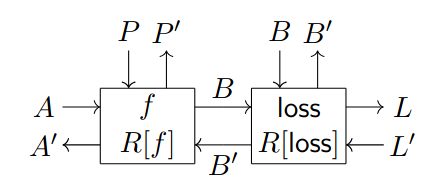
\includegraphics[width=\textwidth]{figures/lenses_model_loss.png}
      \caption{}
    \end{subfigure}
    \begin{subfigure}{0.4\textwidth}
      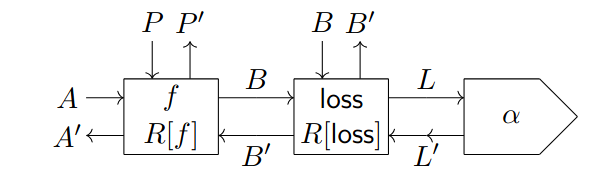
\includegraphics[width=\textwidth]{figures/lenses_model_loss_optimizer.png}
      \caption{}
    \end{subfigure}
    \begin{subfigure}{0.5\textwidth}
      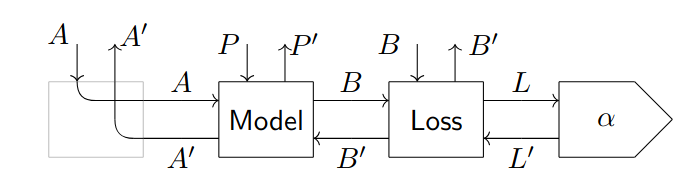
\includegraphics[width=\textwidth]{figures/lenses_supervised_learning1.png}
      \caption{}
    \end{subfigure}   
    \begin{subfigure}{0.5\textwidth}
      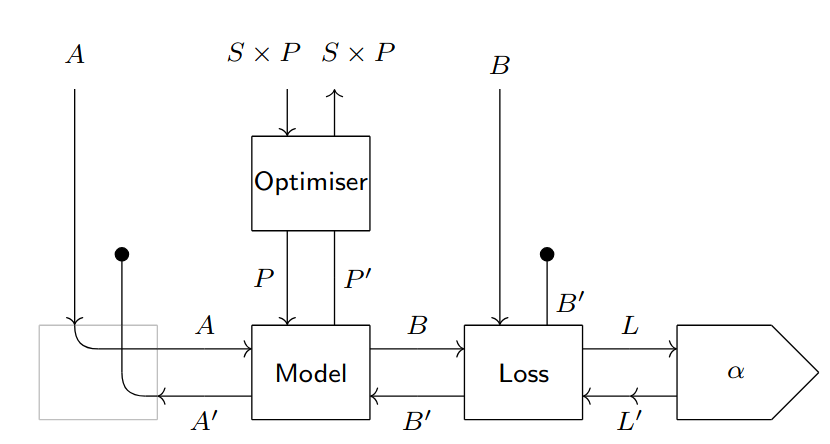
\includegraphics[width=\textwidth]{figures/lenses_supervised_learning2.png}
      \caption{}
    \end{subfigure}                   
    \caption[Supervised learning with parametric lenses]{String diagrams representing (a) the composition of a model lens and an optimizer lens (b) the composition of a model lens, an optimizer lens, and a learning rate lens, (c) a composition of lenses representing a complete supervised learning algorithm, (d) the same lens of the previous point withuseless wires plugged. (Images taken from \cite{cruttwell2022categorical}.)}
    \label{fig: suplearnlenses}
  \end{center}
\end{figure}

It can be helpful to think about dangling wires in the diagrams as open slots where other components can be plugged. For instance, the diagram of \textit{Fig. \ref{fig: suplearnlenses} (a)} has dangling wires labeled with $L$ on its right. We can use a learning rate lens $\alpha$ to link these wires and allow forward-propagating information to "change direction" and go backwards. $\alpha$ must have domain equal to $\left( \begin{smallmatrix} L \\ L \end{smallmatrix} \right)$ and codomain equal to $\left(\begin{smallmatrix} 1 \\ 1 \end{smallmatrix}\right)$, where $1$ is the terminal object of $\mathcal{C}$. For instance, if $\mathcal{C} = \mathbf{Smooth}$, $\alpha$ might just multiply the loss by some $\epsilon$, which is what machine learning practitioners would ordinarily call learning rate. \textit{Fig. \ref{fig: suplearnlenses} (b)} shows how a learning rate can be linked to the loss function and the model using post-composition.


The final element needed for the model $\mathsf{Model}$ in \textit{Fig. \ref{fig: suplearnlenses} (b)} to learn is an optimizer. It is shown in \cite{cruttwell2022categorical} that optimizers can be represented as reparametrisations in $\mathbf{Para}(\mathbf{Lens}(\mathcal{C}))$. More specifically, we might see an optimizer as a lens $\left( \begin{smallmatrix} P \\ P \end{smallmatrix} \right) \to \left( \begin{smallmatrix} Q \\ Q \end{smallmatrix} \right)$. In gradient descent, for example, $P = Q$ and the aforementioned lens is $\left( \begin{smallmatrix} 1_P \\ +_P \end{smallmatrix} \right)$. We can plug such reparametrisation on top of the model to obtain the string diagram in \textit{Fig. \ref{fig: suplearnlenses} (c)}. The diagram shows how the machinery hidden by the $\mathbf{Para}(\mathbf{Lens}(\mathcal{C}))$ can take care of forward propagation, loss computation, backpropagation and parameter updating in a seamless fashion.

In the supervised learning lens in \textit{Fig. \ref{fig: suplearnlenses} (c)}, there are actually has two more dangling wires we do not have any use for: namely, the second input $A$ of the model and the second parameter $B$ of the loss functions. These are not a problem as we can just plug them with delete maps taken from the Cartesian structure of $\mathcal{C}$. We can also bend the input wires with an appropriate lens to turn them into parameters. We are then left with a $\left(\begin{smallmatrix} 1 \\ 1 \end{smallmatrix}\right) \to \left(\begin{smallmatrix} 1 \\ 1 \end{smallmatrix}\right)$ parametric lens with parameter space $\left(\begin{smallmatrix} A \\ 1 \end{smallmatrix}\right) \times \left(\begin{smallmatrix} P \\ P \end{smallmatrix}\right) \times \left(\begin{smallmatrix} B \\ 1 \end{smallmatrix}\right)$. This lens is pictured in \textit{Fig. \ref{fig: suplearnlenses} (d)}.




\subsection{Weight tying, batching, and the learning iteration}

Both \cite{cruttwell2022categorical} and \cite{gavranovic2024fundamental} emphasize the essential role played by weight tying in deep learning. Weight tying can be implemented within the parametric lens framework as a reparametrization that copies a single parameter to many parameter slots (see \textit{Fig. \ref{fig: weighttying}} (a)): given $(P \times P, f): \mathbf{Para}(\mathcal{C})(X,Y)$, we can define $(P, f^{\Delta_P}): \mathbf{Para}(\mathcal{C})(X,Y)$ so that
\[f^{\Delta_P}: P \times X \stackrel{\Delta_P \times X}{\longrightarrow} P \times P \times X \stackrel{f}{\longrightarrow} Y.\]
Weight tying can also be used for batching: batching is implemented by instantiating $n$ different copies of our supervised learning lens (comprised of model, loss function, and learning rate) and tying the parameters to a unique value. Then, it suffices to feed the $n$ data points to the $n$ lenses, and we can optimize across a single parameter (see \textit{Fig. \ref{fig: weighttying}} (b)).

\cite{cruttwell2022categorical} introduces a possible representation for the whole learning iteration of a supervised learning model within the parametric lens framework. The paper suggests extracting the bacward pass of the lens in \textit{Fig. \ref{fig: suplearnlenses} (d)} and reframing it as a $P \to P$ parametric map with parameters $A \times B$. Since this is an endomap, it can be composed $n$ times with itself to obtain a $P \to P$ map, which is proposed as a model of the learning iteration. While this approach requires breaking lenses apart, it is markedly simple.

\begin{figure}[h]
  \begin{center}
    \begin{subfigure}{0.3\textwidth}
      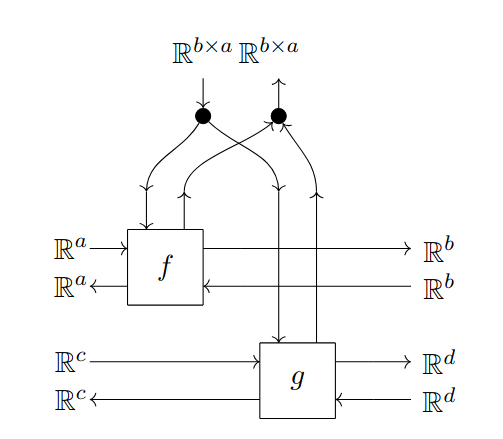
\includegraphics[width=\textwidth]{figures/weight_tying.png}
      \caption{}
    \end{subfigure}
    \begin{subfigure}{0.3\textwidth}
      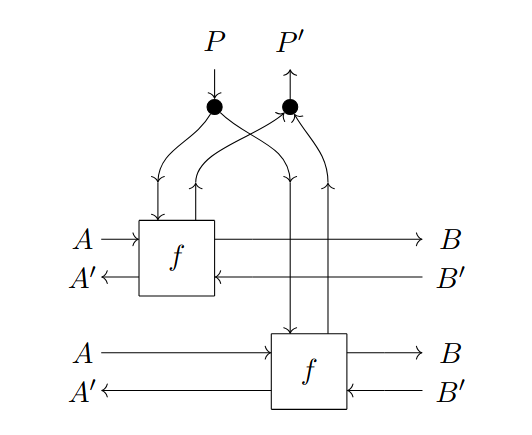
\includegraphics[width=\textwidth]{figures/batching.png}
      \caption{}
    \end{subfigure}              
    \caption[Weight tying and batching]{String diagrams representing (a) weight trying and (b) batching, both implemented using the copy maps of a Cartesian category. (Images taken from \cite{cruttwell2022categorical}.)}
    \label{fig: weighttying}
  \end{center}
\end{figure}


\subsection{Empirical evidence}

Empirical evidence for the effectiveness of the parametric lens framework discussed in this section can be found in \cite{cruttwell2022categorical}, where the authors go on to implement a Python libraries for gradient-based learning based on these ideas. They use the library to develop a MNIST classifier, obtaining comparable accuracy to models developed using traditional tools.


Since parametric lenses can easily be implemented functionally and without side effects, success stories as the one mentioned above foreshadow a future where popular machine learning libraries also follow elegant functional paradigms informed by category theory. Quoting  \cite{cruttwell2022categorical} directly, \lq[the] proposed algebraic structures naturally guide programming practice\rq.


\section{Future directions and related work}

The parametric optic framework discussed in this chapter is very promising, but there is still a lot of work that needs to be done so that it can reach its full potential. For instance, \cite{gavranovic2024fundamental} conjectures that weighted optics can be used in its full generality to model differentiation in cases which are not covered by lenses. For instance, lenses cannot model AD algorithms that do not use gradient checkpointing, while weighted optics are conjectured to be able to do so. \cite{gavranovic2024fundamental} also suggests investigating locally graded categories as potential replacements for actegories, and also investigating the applications of parametric optics to meta-learning, that is deep learning where the optimizers themselves are learned. Moreover, \cite{cruttwell2022categorical} conjectures that some of the axioms of CRDC may be used to model higher order optimization algorithms. Finally, as suggested by \cite{cruttwell2022categorical}, hopefully future work will allow the parametric optic framework to encompass non-gradient based optimizers such as the ones used in probabilistic learning. See \cite{shiebler2021category} for more on this topic.

We conclude this chapter by discussing three other directions of machine learning research that are closely related to the framework of parametric optics.
  

\subsection{Learners}


One of the first compositional approaches to training neural networks in the literature can be found in the seminal paper \cite{fong2019backprop}, which spurred much research in the field, including what is presented in \cite{gavranovic2024fundamental} and \cite{cruttwell2022categorical}. The authors introduce a category of learners, objects which are meant to represent components of a neural network and behave similarly to parametric lenses. 


\begin{definition}[Category of learners]
  Let $A$ and $B$ be sets. A learner $A \to B$ is a tuple $(P, I, U, r)$ where $P$ is a set, and $I: P \times A \to B$, $U: P \times A \times B \to P$, and $r: P \times A \times B \to A$ are functions.
  $P$ is known as parameter space, $I$ as implement functions, $U$ as update function, and $r$ as request function. Two learners $(P, I, U, r): A \to B$ and $(Q, J, V, s): B \to C$ compose forming $(P \times Q, I \ast J, U \ast V, r \ast s ): A \to C$, where
  \[(I \ast J)(p,q,a) = J(q,I(p,a)),\]
  \[(U \ast V)(p,q,a,c) = (U(p,a,s(q,I(p,a),c)), V(q,I(p,a),c)),\]
  \[(r \ast s)(p,q,a,c) = r(p,a,s(q,I(p,a),c)).\]
  Learners quotiented by an appropriate reparametrization relationship\footnote{As argued in \cite{fong2019backprop}, learners could be studied from a bicategorical point of view, where reparametrizations would just be $2$-cells. We could then use a connected component projection to compress $\mathbf{Learn}$ into a $1$-category $\mathbf{Learn}$, as it is done for $\mathbf{coPara}$ when defining weighted optics.} form a category $\mathbf{Learn}$.
\end{definition}

A learner represents an instance of supervised learning: the implement function takes a parameter and implements a function and the update function updates the parameters using a data from a dataset. The request function is necessary to implement backpropagation when optimizing a composition of learners. Suppose we select a learning rate $\epsilon$ and an error function $e: \mathbb{R}^2 \to \mathbb{R}$ such that $y \mapsto \frac{\partial e }{\partial x}(x_0, y)$ is invertible for all $y$. It is argued in \cite{fong2019backprop} that we can define a functor $L_{\epsilon, e}: \mathbf{Para}_{\times}(\mathbf{Smooth}) \to \mathbf{Learn}$ which takes a parametric map and yields an associated learner that implements gradient descent. 


We do not have the space to talk about learners at length, but we wish to draw a short comparison between parametric weighted optics (and, in particular, parametric lenses) and the approach of \cite{fong2019backprop}, given the relevant position held by the paper in the machine learning literature. The similarities between learner-based learning and lens-based learning are evident: every learner $(P, I, U, r)$ looks like a parametric lens, where $I$ passes information forward, $r$ passes information backwards and $P$ is the parameter space. Moreover, the role of $L_{\epsilon, e}$ is very similar to the role played by $\mathbf{Para}(\mathbf{R}_{\mathcal{C}})$ in optic-based learning. Such similarities were even discussed in the original paper \cite{fong2019backprop} and have been researched at length: it has been proved in \cite{fong2019lenses} that learners can be functorially and faithfully embedded in a special category of symmetric lenses (as opposed to the lenses of \textit{Def. \ref{def: lenses}}, which are asymmetric).


Despite the similarities, there is one fundamental difference between the lens-based approach and the learner-based approach: each learner carries its own optimizer, whereas optimization of lenses is usually carried out separately. Moreover, if we compare parametric weighted optics with learners, the latter clearly win in versatility, generality, and (at least from our point of view) conceptual clarity. It is argued in \cite{shiebler2021category} and \cite{cruttwell2022categorical} that the parametric lens framework largely subsumes the learner approach. More information regarding the comparison can also be found in \cite{gavranovic2024fundamental}.


\subsection{Exotic differential categories}

We have presented the parametric weighted optic approach of \cite{gavranovic2024fundamental} and \cite{cruttwell2022categorical} within the context of neural networks for the sake of simplicity, but the framework has been developed with generality in mind and applies to a much wider range of situations. For instance, we can easily replace $\mathbf{Smooth}$ with any other CRDC $\mathcal{C}$, yielding a full-feature compositional framework for gradient-based learning over $\mathcal{C}$.


Switching to a different CRDC is useful because different differential categories can lead to different learning outcomes, both in terms of accuracy of the model and in terms of training computational costs (\cite{wilson2022categories}).
For instance, is argued in \cite{wilson2022categories} that polynomial circuits can be used to define and train intrinsecally discrete machine learning models. Even \lq radical \rq environments such as Boolean circuits - where scalars reside in $\mathbb{Z}_2$ - seem to be conductive to machine learning under the right choice of architecture and optimizer (\cite{wilson2021reverse}). Using such exotic differential categories may be of great advantage because they might be able to better reflect the intrinsic computational limits of computer arithmetics, leading to more efficient learning (\cite{wilson2022categories}). 


\subsection{Functional reverse-mode automatic differentiation}

Finally, we wish to highlight the similarities between the formal theory of differential categories illustrated here and the work in \cite{elliott2018simple}. The paper describes the Haskell implementation of a purely functional automatic differentiation library, which is able to handle both forward mode and backward mode AD without resorting to the mutable computational graphs used by most current day libraries. 

Among the main insights of \cite{elliott2018simple}, it is stated that derivatives should not be treated as simple vectors, but as linear maps, or multilinear maps in the case of uncurried higher-order derivatives. Moreover, the author shows that differentiation can be made compositional by working on pairs $(f, Df)$, which behaved very similarly to lenses. As noted by \cite{shiebler2021category}, however, \cite{cruttwell2022categorical} and other lens-theoretical perspectives do not subsume the work in \cite{elliott2018simple} because of the latter's programming focus. See \cite{shiebler2021category} for more information regarding this comparison.



\clearpage{\pagestyle{empty}\cleardoublepage}




























































\chapter{From Classical Computer Science to Neural Networks}


\lhead[\fancyplain{}{\bfseries\thepage}]{\fancyplain{}{\bfseries\rightmark}}




Classical computer science focuses on discovering algorithms, that is ordered sequences of steps which operate in precisely set, idealized conditions and have strong guarantees of correctness due to their exact mathematical formulations. Neural networks, on the other hand, are able to work in messy, real-world conditions, but offer very so few guarantees of correctness that their performance is often described as \textit{unreasonably} good. Moreover, whereas algorithms generalize very well (most software engineers will only need a few dozen algorithms in their entire career), neural networks are often completely helpless when pitted against out of distribution inputs. Hence, algorithms and neural networks can be seen as complementary opposites (\cite{velivckovic2021neural}, \cite{velivckovic2022clrs}).


Recent attempts going under the label of \textit{neural algorithmic reasoning} (see \cite{velivckovic2021neural} for a very short introduction to the subject) have tried to get the best of both worlds by training neural networks to execute algorithms (see e.g \cite{ibarz2022generalist}). The CLRS benchmark (introduced by \cite{velivckovic2022clrs}) uses graphs to represent the computations associated with a few classical algorithms from the famous CLRS introductory textbook (\cite{cormen2022introduction}) so that graph neural networks (GNNs) can be trained to learn these algorithms. The benchmark has spurred a large amount of research in this direction, with very promising results.


More generally, linking machine learning to classical computer science may unlock interesting advances. For example, recovering neural networks as parametric versions of known algorithms may classify existing architectures in a conceptually clear manner and may even help develop new neural network architectures by taking inspiration from well-researched classical notions. In this chapter, we illustrate two lines of inquiry which use category theory to build such a bridge: \textit{categorical deep learning} and an interesting categorical approach to \textit{algorithmic alignment}. Before treating such topics, we will go on a short tangent categorical tangent regarding (co)algebras and the integral transform.




\section{Categorical toolkit}

\subsection{(Co)algebras}
\label{subsec: algebras}

Algebras and coalgebras are a categorical formalization of the principles of induction and coinduction. Induction and coinduction are fundamental to computer science because they allow us to give precise definitions for many data structures and to formalize recursive and corecursive algorithms on such structures. We will touch on (co)algebras very briefly but we refer interested readers to \cite{jacobs1997tutorial} and \cite{wisbauer2008algebras} for further detail.

\begin{definition}[(Co)algebra over an endofunctor]
  \label{def: endalg}
  Let $F: \mathcal{C} \to \mathcal{C}$ be an endofunctor. An algebra over $F$ is a pair $(A,a)$ where $A: \mathcal{C}$ and $a:\mathcal{C}(F(A),A)$. A coalgebra is a pair $(A,a)$ where $A: \mathcal{C}$ and $a:\mathcal{C}(A,F(A))$. In both cases $A$ is known as carrier set and $a$ as structure map.
\end{definition}

(Co)algebras can also be defined on monads: the only difference between (co)algebras over an endofunctor and (co)algebras over a monad is that the latter also need to be compatible with the monad structure, that is satisfy commutative diagrams that represent coherence conditions (see \cite{gavranovicposition}). (Co)algebras over the same functor can be given a categorical structure by using the following notion of homomorphism.

\begin{definition}[Homomorphisms of (co)algebras over an endofunctor]
  Let $(A,a)$ and $(B,b)$ be algebras over the same endofunctor $F: \mathcal{C} \to \mathcal{C}$. An algebra homomorphism $(A,a)\to (B,b)$ is a map $f: \mathcal{C}(A,B)$ such that the diagram in \textit{Fig. \ref{fig: alghom} (a)} is commutative.


  Now suppose $(A,a)$ and $(B,b)$ are coalgebras. A homomorphism between them is a map $f: \mathcal{C}(A,B)$ such that the diagram in \textit{Fig. \ref{fig: alghom} (b)} is commutative.
\end{definition}

\begin{figure}[h]
  \begin{center}
    \begin{subfigure}{0.25\textwidth}
      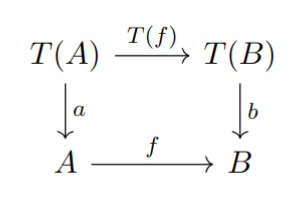
\includegraphics[width=\textwidth]{figures/algebra_hom.png}
      \caption{}
    \end{subfigure}
    \begin{subfigure}{0.25\textwidth}
      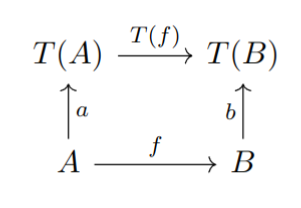
\includegraphics[width=\textwidth]{figures/coalgebra_hom.png}
      \caption{}
    \end{subfigure}   
    \begin{subfigure}{0.25\textwidth}
      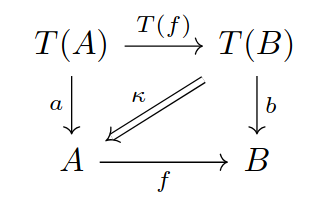
\includegraphics[width=\textwidth]{figures/lax_algebra_hom.png}
      \caption{}
    \end{subfigure}            
    \caption[(Co)algebra homomorphisms]{Conditions under which $f:(A,a)\to(B,b)$ is (a) an algebra homomorphism, (b) a coalgebra homomorphism, (c) a lax algebra homomorphism. (Image (c) is taken from \cite{gavranovicposition}.)}
    \label{fig: alghom}
  \end{center}
\end{figure}


The main intuition behind the notions of algebra and coalgebra is the following: the underlying functor defines a signature for the (co)algebraic structure; the structure of an algebra is a constructor that takes data from $F(A)$ and uses it to build data from $A$, whereas the structure of a coalgebra observes data from $A$ and produces an observation in the form of data from $F(A)$; (co)algebra homomorphism are arrows that preserve the underlying structure. Consider the following clarifying examples from \cite{gavranovicposition}.

\begin{remark}
  In the examples below we use polynomial and exponential expressions to define endofunctors over $\mathbf{Set}$. In this context, $X$ is the argument of the functor, $\times$ is the Cartesian product, $+$ is the disjoint union, $\langle f,g \rangle$ is the pairing induced by $\times$, $[f,g]$ is the pairing induced by $+$, and $B^A$ is the set of functions $A \to B$. The $\times$ operator is assumed to take precedence over the $+$ operator. Similarly, the exponential operator is assumed to take precedence over the $\times$ operator. 
\end{remark}


\begin{example}[Lists]
  \label{ex: lists}
  Let $A$ be a set. Consider the endofunctor $1 + A \times X: \mathbf{Set} \to \mathbf{Set}$. If $\mathsf{List}(A)$ is the set of $A$-labeled lists, $(\mathsf{List}(A), [\mathsf{Nil}, \mathsf{Cons}])$ is an algebra over $1 + A \times X$. Here, $\mathsf{Nil}: 1 \to {List}(A)$ is the map which takes the unique object of $1$ and returns the empty list, while $\mathsf{Cons}: A \times \mathsf{List}(A) \to \mathsf{List}(A)$ is the map which takes an element $a \in A$ and a list $l$ of elements of $A$ and returns the concatenated list $l \cup \{a\}$. The algebra $(\mathsf{List}(A), [\mathsf{Nil}, \mathsf{Cons}])$ describes lists in $\mathsf{List}(A)$ inductively as object formed by concatenating elements of $A$ to other lists in $\mathsf{List}(A)$. The base case is the empty list.
\end{example}

\begin{example}[Mealy machines]
  \label{ex: mealy}
  Now consider two sets $I$ and $O$ of possible inputs and outputs, respectively. Consider the endofunctor $(O \times X)^I: \mathbf{Set} \to \mathbf{Set}$.  Define $\mathsf{Mealy}_{I,O}$ as the set of Mealy machines with inputs and outputs in $I$ and $O$, respectively. Now we can consider the coalgebra $(\mathsf{Mealy}_{I,O}, \mathsf{Next})$, where $\mathsf{Next}$ is the map that takes a Mealy machine $m \in \mathsf{Mealy}_{I,O}$ and yields a function which in turn, given $i \in I$, returns the output of $m$ at $i$ and a new machine $m'$. This is a coinductive description of Mealy machines.
\end{example}

\begin{remark}
  Notice how the description we have given of Mealy machines does not mention the internal states of these objects. This is a recurring aspect of coinductive descriptions: as argued in \cite{jacobs1997tutorial}, coinduction is best interpreted as a process where an observer tracks the behavior of an object from the outside, with no access to its internal state. This is very useful in machine learning because the internal state of a learning model is often unknown or uninterpretable.
\end{remark}

The link between (co)algebras and (co)induction does not stop at the definition level. The example below shows that an algebra homomorphism can model a recursive fold procedure. A similar corecursive unfold procedure can be defined by using a coalgebra homomorphism (see \cite{gavranovicposition} for further detail).

\begin{example}[List folds]
  \label{ex: listfold}
  Consider the algebra $(\mathsf{List}(A), [\mathsf{Nil}, \mathsf{Cons}])$ of lists from \textit{Ex. \ref{ex: lists}}, and consider a second algebra $(Z, [r_0,r_1])$ over the same functor. A homomorphism $f: \mathsf{List}(A) \to Z$ from the former into the latter must satisfy 
  \begin{align*}
    f(\mathsf{Nil}) &= r_0,\\
    f(\mathsf{Cons}(a,l)) &= r_1(a,f(l)). 
  \end{align*}
  Hence, $f$ is necessarily a fold over a list with recursive components $r_0$ and $r_1$. Incidentally, this proves that $f$ is unique, making $(\mathsf{List}(A), [\mathsf{Nil}, \mathsf{Cons}])$ an initial object in the category of algebras over the polynomial endofunctor $1 + A \times X$.
\end{example}

The notion of (co)algebra over a functor can be generalized to the sphere $2$-categories, defining the notion of (co)algebra over a $2$-endofunctor. The basic concepts stay the same but the commutativity of the diagrams definining (co)algebra homomorphisms is relaxed into lax-commutativity. A square diagram of $1$-cells is lax-commutative if there exists a $2$-cell that carries the composition of the top and the right edge onto the composition of the left and bottom edge, as in \textit{Fig. \ref{fig: alghom} (c)}. Once again we refer to \cite{gavranovicposition} for further information.


We conclude the section with the following proposition (\cite{gavranovicposition}), which shows that actegorical strong endofunctors induce $2$-endofunctors over parametric categories. We will use the proposition to study parametric versions of the endofunctors of \textit{Ex. \ref{ex: lists}} and \textit{Ex. \ref{ex: mealy}}.

\begin{proposition}
  \label{prop: paraend}
  Suppose $(\mathcal{C}, \bullet)$ is an $\mathcal{M}$-actegory and $F: \mathcal{C} \to \mathcal{C}$ is an actegorical endofunctor with strength $\sigma$. Then, $F$ induces a  $2$-endofunctor $\mathbf{Para}(F): \mathbf{Para}_{\bullet}(\mathcal{C}) \to \mathbf{Para}_{\bullet}(\mathcal{C})$.
\end{proposition}
\begin{proof}
  Define $\mathbf{Para}(F)$ so that: 
  \begin{enumerate}
    \item $\mathbf{Para}(F)$ acts like $F$ on objects $A: \mathcal{C}$;
    \item $\mathbf{Para}(F)(f) = P \bullet F(A) \stackrel{\sigma_{P,A}}{\longrightarrow} F(P \bullet A) \stackrel{F(f)}{\longrightarrow} F(B)$ for all $(P,f):\mathbf{Para}_{\bullet}(\mathcal{C})(A,B)$;
    \item $\mathbf{Para}(F)$ leaves reparametrizations unchanged.
  \end{enumerate}
\end{proof}


\subsection{Integral transform}

\begin{remark}
  In accordance with the notation of \cite{dudzik2022graph} and \cite{dudzik2024asynchronous}, we use $[A,B]$ to represent the set of $A \to B$ functions, where $A$ and $B$ are sets.
\end{remark}

Suppose $(R, \oplus, \otimes)$ is a commutative semiring. An integral transform is a transformation that carries a function in $[W,R]$ to a function in $[Z,R]$ following a precise chain of steps. Integral transforms\footnote{The label integral transform refers to the fact that similar ideas can be used to write categorical definitions for familiar analytical integral transforms (\cite{golem_ph_utexas_edu}). A similar construct is also used in physics (\cite{eastwood1980cohomology}).} have been introduced by \cite{dudzik2022graph} to provide a single formalism able to describe both dynamic programming and GNNs. Integral transforms can be encoded as polynomial spans.

\begin{definition}[Polynomial span]
  A polynomial span is a triplet $(i: X \to W,p: X \to Y,o: Y \to Z)$ of morphisms in $\mathbf{FinSet}$, the category of finite sets and functions. $i$ is known as input, $p$ as process, $o$ as ouput. $W$ is known as input set, $X$ as argument set, $Y$ as message set, $Z$ as ouput set. We also ask that the fibers of $p$ have total orderings\footnote{Neither we nor \cite{dudzik2022graph} use this requirement but, as stated in the original paper, the requirement is useful to support functions with non-commuting arguments.}. The polynomial span $(i,p,o)$ can be graphically represented as the string diagram in \textit{Fig. \ref{fig: inttransform} (a)}.
\end{definition}

\begin{definition}[Integral transform]
  Let $(R, \oplus, \otimes)$ be a commutative semiring. Let $(i: X \to W,p: X \to Y,o: Y \to Z)$ be a polynomial span. The associated integral transform is the triplet $(i^*: [W,R] \to [X,R], p_{\otimes}: [X,R] \to [Y,R], o_{\oplus}: [Y,R] \to [Z,R])$, where:
  \begin{enumerate}
    \item $i^*$ is the pullback mapping $f \mapsto i \fatsemi f$;
    \item $p_{\otimes}$ is the argument pushforward mapping 
    \[p_{\otimes}(a)(u) = \bigotimes_{e \in p^{-1}(u)}a(e);\]
    \item $o_{\otimes}$ is the message pushforward mapping 
    \[o_{\oplus}(m)(v) = \bigoplus_{e \in o^{-1}(v)}m(e).\]
  \end{enumerate}
  The integral transform $(i^*, p_{\otimes}, o_{\oplus})$ can be represented by the diagram in \textit{Fig. \ref{fig: inttransform} (b)}.
\end{definition}


\begin{figure}[h]
  \begin{center}
    \begin{subfigure}{0.21\textwidth}
      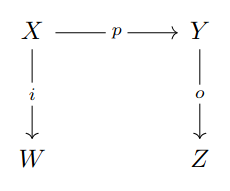
\includegraphics[width=\textwidth]{figures/polynomial_span.png}
      \caption{}
    \end{subfigure}
    \begin{subfigure}{0.28\textwidth}
      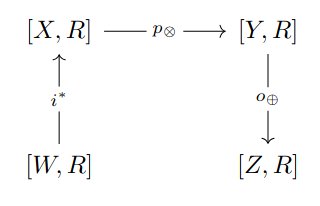
\includegraphics[width=\textwidth]{figures/integral_transform.png}
      \caption{}
    \end{subfigure}            
    \caption[Integral transform]{(a) A polynomial span and (b) the associated integral transform. (Images taken from \cite{dudzik2022graph}.)}
    \label{fig: inttransform}
  \end{center}
\end{figure}


\begin{remark}
  Whereas defining $i^*$ is quite straight-forward, defining $p_{\otimes}$ and $o_{\otimes}$ is more difficult because the arrows $p$ and $o$ point in the wrong direction, which implies that the underlying functions must be inverted before considering the associated pullbacks. However, inverting non-invertible functions yields functions into the powersets of the original domains. Moreover, if we want to preserve the multiplicity of arguments and messages, we have to construct inverses that go into the sets of multisets over the original domains. Hence why we need $\otimes$ and $\oplus$ to aggregate results over such multisets.
  The significance these steps will be clarified later on in this chapter.
\end{remark}



\section{Categorical deep learning}

The optic-based framework we presented in the last chapter provides a structured general-purpose compositional framework for gradient-based learning, but its great versatility has a price: optics are unable to guide the architectural design of our models. It has been shown times and times again that a better architecture makes as much of a difference in machine learning as an algorithm with a better asymptotic cost does in classical computer science. 
Therefore, finding a principled mathematical framework able to guide such architectural choices is of paramount importance. 


Designing an architecture is almost synonymous to imposing a set of constraints: for instance, convolutional layers are notoriously equivalent to translationally equivariant linear layers. Hence, it makes sense to inform the choice of architecture by informing the choice of constraint. Among the various attempts to develop a principled theory of machine learning constraints, \textit{geometric deep learning} (see e.g. \cite{bronstein2021geometric}), or GDL is particularly relevant. Categorical deep learning, or CDL, evolved as categorical generalization of GDL (\cite{gavranovicposition}).


\subsection{From GDL to CDL}

Geometric deep learning focuses on equivariance constraints defined with respect to group actions, according to the following definition.

\begin{definition}[Group action equivariance and invariance]
  \label{def: equivariance}
  Let $G$ be a group and let $(S, \cdot)$ and $(T, \ast)$ be $G$-actions. A function $f: S \to T$ is equivariant with respect to the aforementioned actions if $f(g \cdot s) = g \ast f(s)$ for all $s \in \mathcal{S}$ and for all $g \in \mathcal{G}$. We say that $f$ is invariant if $\ast$ is the trivial action on $T$, and thus $f(g \cdot s) = f(s)$ for all $s$ and $g$.
\end{definition}

The GDL approach prescribes that a desired constraint should be expressed in terms of equivariance with respect to group action so that associated equations can be derived. Solving such equations usually implies tying weights, which reduces the net number of parameters in the models and provides the various advantages (see e.g. \cite{olah2020naturally}) afforded by equivariance.


GLD has been successfully applied in contexts where data transformations can be expressed in group-theoretical terms (see e.g. \cite{bronstein2021geometric}). Regrettably, this is not always the case, as many transformations we can subject the data to are either not invertible or even not compositional (\cite{gavranovicposition}). Moreover, as highlighted in \cite{gavranovicposition}, although GDL is effective at describing the constraints that a model should implement, it is not always clear how such constraints can be actually be implemented since solving the equations associated with a constraint might be extremely challenging.  
Categorical deep learning, introduced by \cite{gavranovicposition}, attempts to solve the aforementioned problems using category theory\footnote{As stated in \cite{bronstein2021geometric}, GDL is inspired by the \textit{Erlangen Programme}, which unified geometry around the notion of invariant at the end of the nineteenth century. Since category theory can be seen as an extension of the \textit{Programme} (as we already remarked in the introduction to this thesis), it is only natural to attempt to generalize GDL by categorical means.} to generalize the notion of equivariance and to tie specific constraints to specific architectures.

\begin{remark}
  At the moment, to the best of our knowledge,  \cite{gavranovicposition} is the only publicly available paper that discusses the ideas of CDL. 
\end{remark}

The main insight of CDL is that group actions can be represented as algebras over the group action monads, and that maps that are equivariant with respect to these actions are homomorphisms between these algebras. Hence, GDL can be generalized by taking into consideration (co)algebras over other monads and endofcuntors. CDL generalizes GDL into a theory of (co)algebras over endofunctors and monads, yielding a "theory of all architectures" (\cite{gavranovicposition}). This profecy has not yet been fulfilled, since only a few architectures have been studied within the framework of CDL at the moment of writing this thesis. However, the results shown in \cite{gavranovicposition} are very promising and, hopefully, future work will widen the scope of CDL to include derivations for more architectures.

The following proposition and the subsequent example show how exactly CDL subsumes GDL.

\begin{proposition}
  Let $(G,e,\cdot)$ be a group. The endofunctor $G \times X: \mathbf{Set} \to \mathbf{Set}$ can be given a monad structure using the natural transformations $\eta$, with components $\eta_S: s \mapsto (e,s)$, and $\mu$, with components $(g,h,s) \mapsto (g \times h, s)$. 
  The monad $(G \times -, \eta, \mu)$ can serve as a signature for $G$-actions. The actions themselves can be recovered by considering algebras $(S,\ast)$ for the monad, and, given two actions $(S,\ast)$ and $(T,\star)$, an associated equivariant map $f: S \to T$ is a $(S,\ast) \to (T,\star)$ monad algebra homomorphism.
\end{proposition}
\begin{proof}
  It suffices to compare the equations that define group actions and group action invariance with the commutative diagrams in \textit{Fig. \ref{fig: alghom}}.
\end{proof}

\begin{example}[Linear equivariant layer]
  \label{ex: translationaction}
  Consider a carrier set $S = \mathbb{R}^{\mathbb{Z}_2}$, which can be seen as a pair of pixels. Consider the translation action $(i \ast s)(j) = s(i-j)$ of $G = \mathbb{Z}_2$ on $S$, which can be seen as swapping the pixels.
  We want to find a linear map $f: S \to S$ which is equivariant with respect to the action. Imposing the equivariance constraints as equations on the entries of the matricial representation $W_f \in \mathbb{R}^{2 \times 2}$ of the map, we can prove that $f$ is equivariant if and only if $W_f$ is symmetric (\cite{gavranovicposition}).
\end{example}


\subsection{(Co)inductive definitions for RNNs}

As seen in \textit{Ex. \ref{ex: translationaction}}, the formalism of CDL subsumes the formalism of GDL, but the difference between the two is not a simple matter of notation: CDL is much more general. The most significant piece of novel contribution delineated in \cite{gavranovicposition} is the use of (co)algebras and (co)algebra homomorphisms over parametric categories to (co)inductively define recurrent neural networks (GNNs) and recursive neural networks (TreeRNNs). (Co)algebras are used to define cells, whereas the associated homomorphisms provide the weight-sharing mechanics used to unroll them. Let us build on \textit{Ex. \ref{ex: lists}} and \textit{Ex. \ref{ex: listfold}}, as is done in \cite{gavranovicposition}.

\begin{example}[Folding recurrent neural network cell]
  \label{ex: frnncell}
  Consider the endofunctor $1 + A \times X: \mathbf{Set} \to \mathbf{Set}$ from \textit{Ex. \ref{ex: lists}}. Consider the Cartesian action of $\mathbf{Set}$ on itself and associate the following actegorical strength to the functor: $\sigma_{P,X}(p,\mathrm{inl}) = \mathrm{inl}$ and  $\sigma_{P,A}(p,\mathrm{inr}(x,x')) = \mathrm{inr}((p,x), (p,x'))$. Now that the functor is actegorical strong, we can use \textit{Prop. \ref{prop: paraend}} to construct an endofunctor $\mathbf{Para}(1 + A \times X): \mathbf{Para}_{\bullet}(\mathbf{Set}) \to \mathbf{Para}_{\bullet}(\mathbf{Set})$. Consider an algebra $(S,(P,\mathsf{Cell}))$ for this functor. Via the isomorphism $P \times (1 + A \times X) \cong P + P \times A \times X$, we deduce that $\mathsf{Cell} = [\mathsf{Cell}_0, \mathsf{Cell}_1]$, where $\mathsf{Cell}_0: P \to S$ and  $\mathsf{Cell}_1: P \times A \times S \to S$. We can interpret $\mathsf{Cell}_0$ and $\mathsf{Cell}_1$ as folding recurrent neural network cells: $\mathsf{Cell}_0$ provides the initial state based on its parameter and $\mathsf{Cell}_1$ takes in the old state, a parameter, and an input, which are then used to return a new state (\textit{Fig. \ref{fig: foldingrnn} (a)}).
\end{example}

\begin{example}[Unrolling of a folding recurrent neural network]
  \label{ex: frnnunroll}
  Use \textit{Prop. \ref{prop: embeddingth}} to embed the list algebra $(\mathsf{List}(A), [\mathsf{Nil}, \mathsf{Cons}])$ from \textit{Ex. \ref{ex: lists}} as an algebra over the endofunctor $\mathbf{Para}(1 + A \times X)$ define in \textit{Def. \ref{ex: frnncell}}. Now consider an algebra homomorphism $(P,f): (\mathsf{List}(A), [\mathsf{Nil}, \mathsf{Cons}]) \to (S,(P,\mathsf{Cell}))$. Since we are working with algebras over a $2$-endofunctor, we also need to specify a $2$-cell that makes the homomorphism diagram (\textit{Fig. \ref{fig: alghom} (c)}) lax-commutative. Using the weight-tying reparameterization $\Delta_P$ yields the lax commutative diagram in \textit{Fig. \ref{fig: foldingrnncommdiag}}, which uniquely identifies $f$ as the fold function which takes a list of inputs in $A$ and unrolls a folding recurrent neural network that reads such inputs. The weight-tying reparametrization makes sure that each cell of the unrolled network uses the same parameters (see \textit{Fig. \ref{fig: foldingrnn} (b)} for a graphical representation). 
\end{example}

\begin{figure}[h]
  \begin{center}
    \begin{subfigure}{0.3\textwidth}
      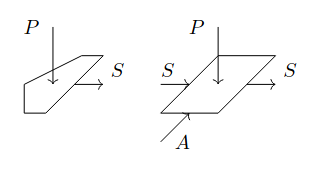
\includegraphics[width=\textwidth]{figures/folding_rnn_cell.png}
      \caption{}
    \end{subfigure}
    \begin{subfigure}{0.48\textwidth}
      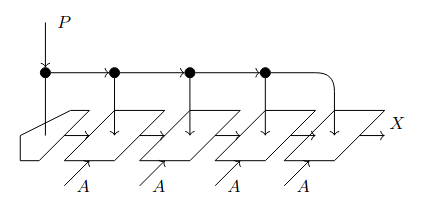
\includegraphics[width=\textwidth]{figures/folding_rnn.png}
      \caption{}
    \end{subfigure}            
    \caption[Folding RNN]{(a) Two kinds of folding RNN cell represeting the initial state of the network and a generic state update based on input. (b) A folding RNN unrolled using weight tying. (Images taken from \cite{gavranovicposition}.)}
    \label{fig: foldingrnn}
  \end{center}
\end{figure}

\begin{figure}[h]
  \begin{center}
    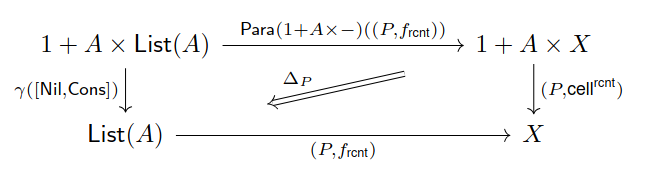
\includegraphics[width=0.6\textwidth]{figures/folding_rnn_lax_diagram.png}     
    \caption[Lax-commutative diagram for the unrolling of a folding RNN]{ Lax-commutative diagram that makes $(P,f): (\mathsf{List}(A), [\mathsf{Nil}, \mathsf{Cons}]) \to (S,(P,\mathsf{Cell}))$ an algebra homomorphisms. (Image taken from \cite{gavranovicposition}.)}
    \label{fig: foldingrnncommdiag}
  \end{center}
\end{figure}



The construction in  \textit{Ex. \ref{ex: frnncell}} and \textit{Ex. \ref{ex: frnnunroll}} constitutes a precise mathematical link between the classical data structure of lists and the machine learning construct of folding RNNs. Similarly, \cite{gavranovicposition} recovers recursive neural networks (TreeRNNs) by building upon classical binary trees and, even more interestingly, complete RNNs are recovered from the coalgebra of \textit{Ex. \ref{ex: mealy}}, which reveals an interesting link between RNNs and Mealy machines. This begs the question: if Mealy machines generalize to recurrent neural networks, what do Moore machines generalize to? It is argued in the paper that they generalize to a variant of RNN where different cells (which share the same weights) are used for state update and output production. Hopefully, more work in this direction will lead to new NN architectures inspired from other classical concepts. \textit{Fig. \ref{fig: cells}} shows various kinds of NN cells and the endofunctors used in their (co)algebraic definitions.

\begin{remark}[CDL and optic-based learning]
  In all the examples discussed above, the (co)algebra homomorphisms in question return parametric maps $(P,\mathsf{model})$, which we can interpret as untrained NN models. We can feed these maps into the $\mathbf{R}_{\mathcal{C}}$ functor associated with a generalized Cartesian reverse differential category\footnote{The examples illustrated in this section have been developed in $\mathbf{Set}$, but we see no reason why they couldn't be specialized to an appropriate CRDC.} to augment them with their reverse derivative. The framework of parametric lenses described in 
  \textit{Sec. \ref{sec: opticbasedlearning}} can then be used to train these networks. CDL and optic-based learning are thus compatible and even complementary.
\end{remark}

\begin{figure}[h]
  \begin{center}
    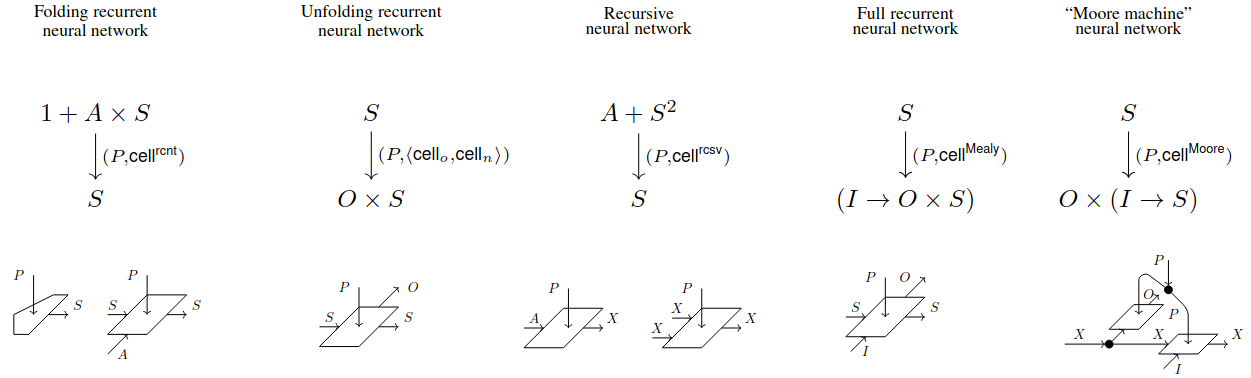
\includegraphics[width=\textwidth]{figures/cells.png}     
    \caption[Neural network cells]{Various kinds of NN cells and the endofunctors used in their (co)algebraic definitions. (Image taken from \cite{gavranovicposition}.)}
    \label{fig: cells}
  \end{center}
\end{figure}

\section{Algorithmic alignment: GNNs and dynamic programming}


One of them main tenets of neural algorithmic reasoning is \textit{algorithmic alignment} (\cite{xu2019can}), that is, the presence of structural similarities between the subroutines of a particular algorithm and the architecture of the neural network selected to learn such algorithm.
Since \cite{xu2019can} has shown that dynamic programming algorithms align very well with GNNs, and since dynamic programming encompasses a wide variety of techniques algorithms to many different domains, GNNs  are at the forefront of neural algorithmic reasoning research (\cite{dudzik2022graph}). However, the exact link between GNNs and dynamic programming has yet to be fully formalized. In this section we present the work of \cite{dudzik2022graph}, which attempts to derive such a formalization, and the work in \cite{dudzik2024asynchronous}, which studies conditions under which GNNs are invariant with respect to various form of asynchrony\footnote{While much of the work described in \cite{dudzik2024asynchronous} does not fall under the umbrella of applied category theory, we still mention it because on its close link with the work of \cite{dudzik2022graph} and with the idea of algorithmic alignment. Hopefully, future work will explore the intersection between this work and category theory.}, which is argued to improve algorithmic alignment in some cases.


\subsection{Integral transforms for GNNs and dynamic programming}

The main link between dynamic programming and GNNs is that dynamic programming itself can be interpreted from a graph-theoretical point of view. Dynamic programming breaks up problems into subproblems recursively until trivial base cases are reached. We can thus consider the graph with nodes corresponding to subproblems and edges $(y,x)$ corresponding to the relationships \lq $y$ is a subproblem of $x$ \rq. Then, the solutions of the subproblems are recusrively recombined to solve the original problem. This dynamic is very similar to message passing: the simpler cases are solved first, and their solutions are passed as messages along the edges so that they can be used to solve more complex cases. The architecture of a graph neural network usually implements such a message passing dynamic. However, rigorously formulating the link between the architecture of GNN and the structure an associated dynamic programming algorithm is not easy, the main obstacle being the difference in data type handled by the two mathematical processes: dynamic programming usually deals with tropical objects such as the semiring $(\mathbb{N} \cup \{\infty\}, \min, +)$, while GNNs usually deal with linear algebra over $\mathbb{R}$ (\cite{dudzik2022graph}).

\cite{dudzik2022graph} proposes the formalism of integral transforms as the common structure behind both GNNs and dynamic programming. While a full formal proof is not given, the idea is illustrated by showing that both the Bellman-Ford algorithm and the message passing neural network (MPNN) architecture can be expressed with the help of integral transforms. The difference in data type is overcome by using the weakest common hypothesis: that the data and associated operations form a semiring.


\subsubsection{Bellman-Ford algorithm}

The Bellman-Ford (BF) algorithm is one of the most popular dynamic programming algorithms and is used to find the shortest paths between a single starting node and every other node in a weighted graph $G = (V, E)$. Since we can see every node of the graph as a subproblem, and since we can see the associated edges as subproblem relationships, the BF algorithm is a very good candidate for a GNN implementation. The algorithm operates within the tropical min-plus semiring $(R = \mathbb{N} \cup \{\infty\}, \oplus = \min, \otimes = +)$, and the data can be provided as a tuple $(d, b, w)$ of three functions into $R$. Here, $d: V \to R$ stores the current best distances of the nodes, $b: V \to R$ stores the weights of the nodes, and $w: E \to R$ stores the weights of the edges. $d$ is initialized as the function that maps the initial node to $0$ and every other node to $\infty$. The values of $d$ are updated at each step of the algorithm according to the following formula, where $\mathcal{N}_u = \{v \text{ s. t. } (v,u) \in E\}$ represent the one-hop neighborhood of a node $u$:
\[d_u \longleftarrow  \min\left(d_u, \min_{v \in \mathcal{N}_u}(d_v) + w_{v,u}\right).\]


\cite{dudzik2022graph} propose the integral transform encoded by the polynomial span in \textit{Fig. \ref{fig: polyspans} (a)} as the supporting structure of the BF algorithm. The functions $i$, $p$, and $o$ are defined as follows:
\begin{enumerate}
  \item $i: (V + E) + (V + E) \to V + (V + E)$ acts as the identity on the first $V$, it maps the edges of the first $E$ to their sources, and it acts as the identity on the second $V + E$ pair;
  \item $p: (V + E) + (V + E) \to V + E$ just collapses the two copies of $V + E$;
  \item $o$ acts as the target function on the $E$ and as the identity on $V$.
\end{enumerate}
It is argued in the paper that the whole integral transform acts as step of the algorithm, carrying the data in $(d, b, w)$ to the updated function $d$. Let's examine each step: the input pullback extracts the distances the sources of every edge; the argument pushforward computes the lengths of the one-hop extensions of the known shortest paths (the weight of each node is treated as the weight of a self-edge in this case); finally, the message pushforward selects the shortest paths to each node among the ones studied by the argument pushforward. 
Hence, the simple polynomial span in \textit{Fig. \ref{fig: polyspans} (a)} successfully encode the whole BP algorithm without any information loss or ad hoc choice. 

\begin{figure}[h]
  \begin{center}
    \begin{subfigure}{0.45\textwidth}
      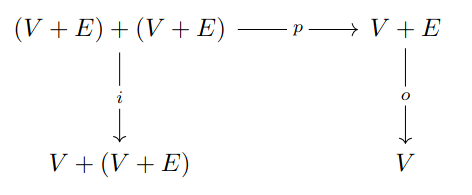
\includegraphics[width=\textwidth]{figures/poly_span_bellman_ford.png}
      \caption{}
    \end{subfigure}
    \begin{subfigure}{0.4\textwidth}
      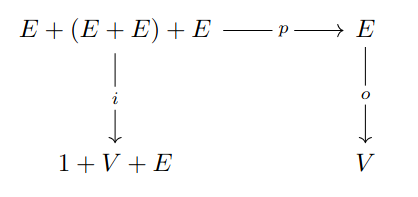
\includegraphics[width=\textwidth]{figures/poly_span_message_passing.png}
      \caption{}
    \end{subfigure}            
    \caption[Bellman-Ford algorithm and message passing networks]{Polynomial spans used to by \cite{dudzik2022graph} to model (a) the Bellman-Ford algorithm and (b) a message pasing neural network. (Images taken from \cite{dudzik2022graph}.)}
    \label{fig: polyspans}
  \end{center}
\end{figure}

\subsubsection{Message passing neural network}

A message passing neural network (MPNN) is a graph neural network described by the following equations (\cite{pmlr-v70-gilmer17a}):
\begin{align*}
  m_v^{t+1} &= \sum_{w \in \mathcal{N}_v}M_t(h_v^t,h_w^t,e_{v,w}),\\
  h_v^{t+1} &= U_t(h_v^t,m_v^{t+1}),\\
\end{align*}
where $t$ represents the time step, and $M_t$ and $U_t$ are learned differentiable functions.


\cite{dudzik2022graph} argues that an MPNN layer can be implemented as the integral transform associated with the polynomial span of \textit{Fig. \ref{fig: polyspans} (b)}, with an extra MLP. Here,
\begin{enumerate}
  \item $i$ sends the first $E$ to $1$, it acts as source and target on the second $E$ and third $E$ respectively, and it acts as the identity on the fourth $E$;
  \item $p$ collapses four $E$'s into one;
  \item $o$ acts as the target function.
\end{enumerate}
In the associated integral transform, $i^*$ gathers graph, features, node features and edge features, $p_{\otimes}$ "projects" the such features on the edges, the MLP combines them, and, finally, $o_{\oplus}$ sends them to the right target.


Although not a perfect representation of the target architecture (due to the extra MLP), the polynomial span in \textit{Fig. \ref{fig: polyspans} (b)} can be used to inform the design of new architectures which are obtained by simple manipulations of the arrows or objects in the diagram. For instance, \cite{dudzik2022graph} uses the integral transform formalism to investigate possible performance improvements on CLRS benchmark tasks (\cite{velivckovic2022clrs}). They consider messages that reduce over intermediate nodes they show these architectures lead to better average performance on these tasks, likely a result of better algorithmic alignment.


\subsection{Asynchronous algorithmic alignment}

\cite{dudzik2024asynchronous} derives conditions under which synchronous GNNs are invariant under asynchronous execution. This is relevant because, as stated in the paper, in many dynamic programming tasks modeled by graphs, only small parts of the aforementioned graphs are changed at each step. A synchronously executed GNN that is trained on these tasks must learn the identity function many times over, which leads to brittleness and wasted computational resources. However, implementing many algorithms that are invariant under asynchronous execution as synchronous GNNs that are also invariant under asynchronous execution leads to better algorithmic alignment and thus more robust and efficient learning.

The authors of \cite{dudzik2024asynchronous} revise the model explored in \cite{dudzik2022graph} so that it includes a message function $\psi$ that generates messages based on gathered arguments (see \textit{Fig. \ref{fig: messagepassing} (a)} for the update diagram). Moreover, the authors argue that it is best to consider GNNs where every graph component that has a persistent state is elevated to the status of node, whereas transient computations are carried out along edges. The resulting GNN can be described by the diagram in \textit{Fig. \ref{fig: messagepassing} (b)}, where $\phi$ is the transit function that updates the persistent state of each node, and $\delta$ is the function that computes the arguments needed to generate the next messages.

\begin{figure}[h]
  \begin{center}
    \begin{subfigure}{0.4\textwidth}
      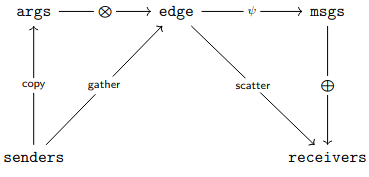
\includegraphics[width=\textwidth]{figures/message_passing_network1.png}
      \caption{}
    \end{subfigure}
    \hfill
    \begin{subfigure}{0.45\textwidth}
      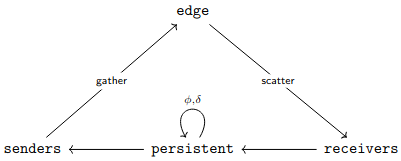
\includegraphics[width=\textwidth]{figures/message_passing_network2.png}
      \caption{}
    \end{subfigure}            
    \caption[Graph neural network architecture]{Diagrams describing the GNN architecture described in \cite{dudzik2024asynchronous}. (Images taken from \cite{dudzik2024asynchronous}.)}
    \label{fig: messagepassing}
  \end{center}
\end{figure}

It is argued in \cite{dudzik2024asynchronous} that invariance under asynchrony can be modeled by giving both arguments and messages monoidal structures. For instance, let $(M, 1, \cdot)$ be the message monoid and let $(A, 0, +)$ be the argument monoid. Then, if $S$ is the set of persistent states, state update and argument generation can be modeled as a function $M \times S \to S \times A$ which maps $(m,s) \mapsto (m \bullet s, \delta_m(s))$. Invariance under asynchronous message aggregation is obtained by defining $\bullet$ as a monoidal action of $M$ on $S$. However, \cite{dudzik2024asynchronous} shows that this is meaningful if and only if the argument generation function $\delta$ is compatible with the unitality and associativity equations of the action. This can only happen if $\delta: m \mapsto \delta_m$ is a $1$-cocycle.

\begin{definition}[$1$-cocycle]
  A map $\delta: M \to [S,A]$ is a $1$-cocycle if and only if the following are satisfied:
  \begin{enumerate}
    \item $\delta_1(s) = 0$ for all $s \in S$;
    \item $\delta_{n \cdot m}(s) = \delta_{n}(m \cdot s) + \delta_m(s)$ for all $s \in S$.
  \end{enumerate} 
  \label{def: cocycle}
\end{definition}

\begin{proposition}
  The state update function $\delta$ described above is asynchronous with respect to message passing if and only if it is a $1$-cocycle.
\end{proposition}

\cite{dudzik2024asynchronous} also proves the following.

\begin{proposition}
  Under the hypotheses described above, a single-input message function $\psi$ supports asynchronous invocation if and only if $\psi$ is a homomorphism of monoids.
\end{proposition}

We will not describe the whole formalism of \cite{dudzik2024asynchronous}, but we will show (without proof) its implications on GNN architecture design. 

\begin{example}
  Consider the GNN architecture:
  \[x_u' = \phi\left(x_u, \bigoplus_{v \in \mathcal{N}_u}\psi(x_{u},x_{v})\right),\]
  where $\oplus$ is a message aggregator function. The authors of \cite{dudzik2024asynchronous} derive conditions under which this architecture is invariant under asynchronies in message aggregation, node update, and argument generation: the GNN is trivially invariant under asynchronous message aggregation if messages $(M,0,\oplus)$ are given a commutative monoidal structure; invariance under asynchronies in node updates is obtained by selecting an update function $\phi$ which sastifies the associative law $\phi(s,m \oplus n) = \phi(\phi(s,m),n)$ for all $m,n \in M$ and for all $s \in S$; finally, invariance under argument generation is obtained if $\phi$ satisfies the $1$-cocycle equations (\textit{Def. \ref{def: cocycle}}). \cite{dudzik2024asynchronous} also gives sufficient conditions that ensure that the $1$-cocycle equations as well as the associative law are true: it suffices that $M=A=S$ and that $\phi=\oplus$ is idempotent.
\end{example}




\section{Future directions and related work}

In this section we provide a brief introduction to the theory of differentiable causal computations and the theory of sheaf neural networks. These two lines of work are adjacent to the main theme of this chapter - relating classical computer science to modern machine learning - and they highlight possible directions for future research into categorical deep learning and the application of integral transforms to neural networks.

\subsection{Differentiable causal computations}

\cite{sprunger2019differentiable} studies the differential properties of causal computations offering valuable insight into the formal properties of recurrent neural networks (RNNs). The paper focuses on sequences $\{f_k\}_{k=0,1,\dots}$ of functions $f_k: S_k \times X_k \to S_{k+1} \times Y_k$ which represent computations executed in discrete time $k$, where, at each tick $k$ of the clock, $f_k$ takes an input $x_k$ and the previous state $s_k$, and uses this data to compute an output $y_k$ and a new state $s_{k+1}$. In symbols, $f_k(s_k,x_k) = (s_{k+1},y_k)$. Such sequences are given a nice compositional structure using the formalism of double categories.

\begin{definition}[Category of tiles]
  Let $\mathcal{C}$ be a Cartesian category. Define $\mathbf{Dbl}(\mathcal{C})$ as the double category with the following data:
  \begin{enumerate}
    \item there is only on $0$-cell, which we represent with the symbol $\cdot$;
    \item the horizontal and vertical $1$-cells are the objects of $\mathcal{C}$;
    \item a $2$-cell (tile) with horizontal source $S$, horizontal target $S'$, vertical source $X$, and vertical target $Y$ is a morphism $f: S \times X \to S' \times Y$ which we represent with the symbol $f:X \overset{S}{\underset{S'}\longrightarrow} Y$.
  \end{enumerate}
  It is handy to also represent $2$-cells $f$ as the tile string diagrams in \textit{Fig. \ref{fig: tiles} (a)}. The horizontal and vertical composition laws for $2$-cells are given consistently with the tile diagrams.
\end{definition}

\begin{definition}[Category of stateful morphism sequences]
  Let $\mathcal{C}$ be a Cartesian category. Define $\mathbf{St}(\mathcal{C})$ as the category with the following data:
  \begin{enumerate}
    \item the objects of $\mathbf{St}(\mathcal{C})$ are sequences $\mathbf{X} = \{X_k\}_{k = 0,1,\dots}$ of objects of $\mathcal{C}$;
    \item the morphisms $\mathbf{X} \to \mathbf{Y}$ are pairs $(\mathbf{f}, i)$, where $\mathbf{f} = \{f_k\}_{k = 0,1,\dots}$ is a sequence of tiles in $\mathbf{Dbl}(\mathcal{C})$ such that $f_k: X_k \overset{S_k}{\underset{S_{k+1}}\longrightarrow} Y_k$, for some sequence $\mathbf{S}$ of states, and $i: 1 \to S_0$ selects an initial state. 
  \end{enumerate}
  The morphisms of $\mathbf{St}(\mathcal{C})$ are known as stateful morphisms sequences and are represented using string diagrams as in \textit{Fig. \ref{fig: tiles} (b)}.
\end{definition}

Stateful morphisms sequences can be truncated and unrolled as one would expect, and it is proved in \cite{sprunger2019differentiable} that there is a bijection between stateful morphism sequences in $\mathbf{St}(\mathbf{Set})([A],[B])$ and causal functions $A^{\mathbb{N}} \to B^{\mathbb{N}}$ (here $[A]$ is the constant sequence of objects $\{A,A,A,\dots\}$). More generally, given any $\mathbf{St}(\mathcal{C})$, we can restrict our attention to constant sequences $[A]$ and stateful sequences of morphisms in the form $([f],i)$, where $f:X \overset{S}{\underset{S}\longrightarrow} Y$ is a tile in $\mathbf{Dbl}(\mathcal{C})$. This yields a subcategory $\mathbf{St}_0(\mathcal{C})$ whose morphisms can be thought of as Mealy machines that take in an input and produce an output based on an internal state which is updated after every computation. The new state is in a sense fed back to the machine after the computation so that a new computation can take place. This is represented by the diagram in \textit{Fig. \ref{fig: tiles} (b)}.


\begin{figure}[h]
  \begin{center}
    \begin{subfigure}[c]{0.3\textwidth}
      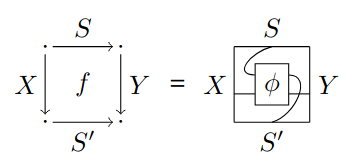
\includegraphics[width=\textwidth]{figures/tiles.png}
      \caption{}
    \end{subfigure}
    \begin{subfigure}[c]{0.45\textwidth}
      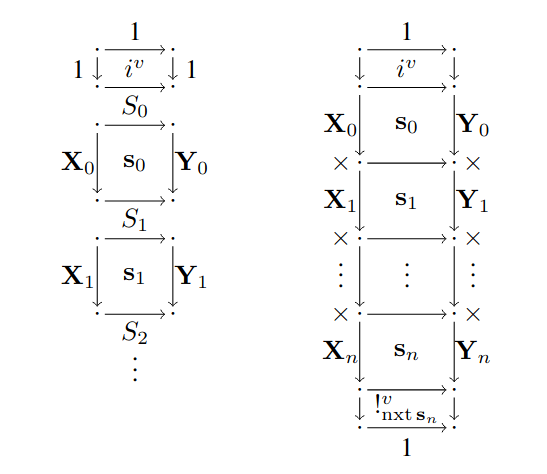
\includegraphics[width=\textwidth]{figures/stateful_morphism_sequences.png}
      \caption{}
    \end{subfigure}            
    \caption[Tiles and stateful morphisms]{(a) String diagrams for a tile in $\mathbf{Dbl}(\mathcal{C})$. (b) String diagrams for a stateful morphism in $\mathbf{St}(\mathcal{C})$ and one of its truncation. (Images taken from \cite{sprunger2019differentiable}.)}
    \label{fig: tiles}
  \end{center}
\end{figure}


The authors of \cite{sprunger2019differentiable} go on to define a delayed trace operation which provides a rigorous formalization of feedback loops such as the one in \textit{Fig. \ref{fig: differentiationanddelayedtrace} (a)}. As stated in the paper, the delayed trace operator is closely related to the more popular trace operator (\cite{joyal1996traced}) and shares many of the same properties. 
Finally, the authors of \cite{sprunger2019differentiable} show how both $\mathbf{St}(\mathcal{C})$ and $\mathbf{St}_0(\mathcal{C})$ can be given the structure of a CDC (\textit{Def. \ref{def: cdc}}), as long as $\mathcal{C}$ is itself a CDC. This differential structure is conceptually clear, rigorously defined, and compatible with the dealyed trace operator. We do not have space to describe the details of these definitions, but we report the relevant string diagrams in \textit{Fig. \ref{fig: differentiationanddelayedtrace} (b),(c)}.


\begin{figure}[h]
  \begin{center}
    \begin{subfigure}{0.3\textwidth}
      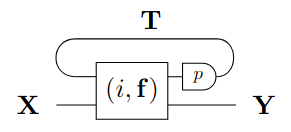
\includegraphics[width=\textwidth]{figures/delayed_trace.png}
      \caption{}
    \end{subfigure}
    \begin{subfigure}{0.45\textwidth}
      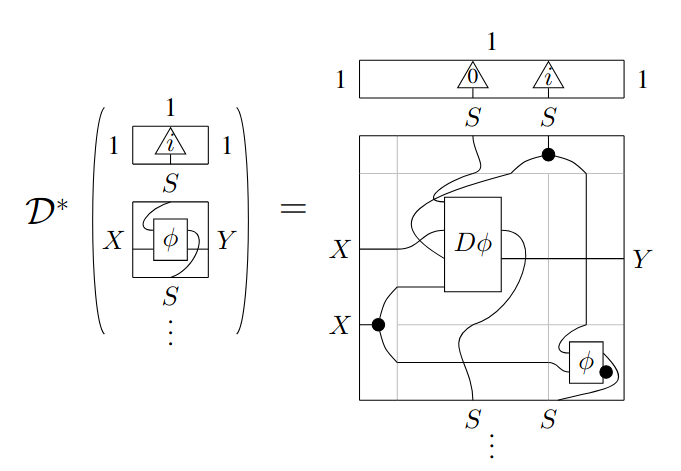
\includegraphics[width=\textwidth]{figures/differentiation_of_stateful_morphism.png}
      \caption{}
    \end{subfigure}
    \\[1cm]
    \begin{subfigure}{0.5\textwidth}
      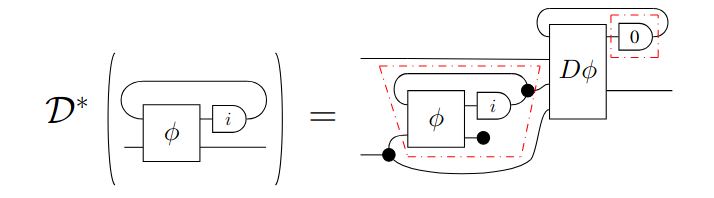
\includegraphics[width=\textwidth]{figures/differentiation_of_delayed_trace.png}
      \caption{}
    \end{subfigure}           
    \caption[Delayed trace and derivatives in $\mathbf{St}_0(\mathcal{C})$]{String diagrams (a) representing a delayed trace in $\mathbf{St}(\mathcal{C})$ as a delayed feedback loop, (b) representing the derivative of a morphism in $\mathbf{St}_0(\mathcal{C})$, (c) representing the derivative of a delayed trace in $\mathbf{St}_0(\mathcal{C})$. (Images taken from \cite{sprunger2019differentiable}.)}
    \label{fig: differentiationanddelayedtrace}
  \end{center}
\end{figure}


The work in \cite{sprunger2019differentiable} provides a theoretical foundation for the technique of backpropagation through time (BPTT), which consists in computing the gradient of the $k$-th unrolling of a RNN in place of the gradient of the such RNN at discrete time $k$. Despite the alleged ad hoc nature of BPTT, \cite{sprunger2019differentiable} proves that the technique does not just \lq involve differentiation \rq but is an actual \lq form of differentiation \rq that can be reasoned about in the formalism of CDCs. Nevertheless, as stated in the paper, the differential operator of $\mathbf{St}(\mathcal{C})$ does not compute explicit gradients, and deriving the latter would from the former would be computationally intractable when there are millions of parameters. 


It is interesting to compare the approach of \cite{sprunger2019differentiable} with the framework of categorical deep learning: both CDL and the work in \cite{sprunger2019differentiable} synthetically describe RNN architectures, but, while CDL focuses on weight sharing mechanics and the coinductive nature of the definition, \cite{sprunger2019differentiable} focuses the differential properties of these architectures. However, neither categorical framework deals with the problems that come up when computing gradients of unrolled RNNs, such as vanishing or exploding gradients (see e.g. \cite{hanin2018neural}). 


\subsection{Sheaf neural networks}

The theory of sheaf neural networks (\cite{hansen2020sheaf}, \cite{bodnar2022neural}, \cite{zaghen2024nonlinear}), or SNNs, is informed by both topology and category theory and aims to improve the GNN architecture by endowing graphs with cellular sheaf structures. In particular, SNNs are designed to solve two main issues that are encountered when training GNNs: oversmoothing, which is the tendency of deep GNNs to spread information too far in the graph to be able to effectively classify nodes, and poor performance on heterophilic graphs, that is graphs where the nodes features are diverse in structure and attributes.

\begin{definition}[Cellular sheaf]
  A cellular sheaf $\mathcal{F}$ associated with a graph $G = (E,V)$ consists of the following data:
  \begin{enumerate}
    \item a vector space $\mathcal{F}(v)$ for every node $v \in V$;
    \item a vector space $\mathcal{F}(e)$ for every edge $e \in E$;
    \item a linear map $\mathcal{F}_{v \trianglelefteq e}: \mathcal{F}(v) \to \mathcal{F}(e)$ for each incident node-edge pair $v \trianglelefteq e$.
  \end{enumerate}
  The vector spaces associated to nodes and edges are known as stalks. The linear maps associated to incident node-edge pairs are known as restriction maps. The direct sum $C^0(G, \mathcal{F})$ of all node stalks is known as space of $0$-cochains, and the direct sum $C^1(G, \mathcal{F})$ of all edge stalks is known as space of $1$-cochains.
\end{definition}

As stated in \cite{zaghen2024nonlinear}, the  node stalks assigned by $\mathcal{F}$ serve as spaces for node features, while the restriction maps allow the data that resides on adjacent nodes to interact on edge stalks. Given a cellular sheaf $\mathcal{F}$, we can define a coboundary map $\delta$ which measures the amount \lq disagreement \rq\footnote{There is a close link between the theory of SNNs and the theory of opinion dynamics. See \cite{zaghen2024nonlinear} for further information.} between nodes. The coboundary map can then be used to define a sheaf Laplacian which can be used to propagate information in the graph.

\begin{definition}[Coboundary map]
  Let $\mathcal{F}$ be a cellular sheaf on a directed graph $G = (E,V)$. The coboundary map associated with $\mathcal{F}$ is the linear map $\delta: C^0(G, \mathcal{F}) \to C^1(G, \mathcal{F})$ that maps $\delta(\mathbf{x})_{e} = \mathcal{F}_{v \trianglelefteq e}(x_v) - \mathcal{F}_{u \trianglelefteq e}(x_u)$ for each edge $e: u \to v$.
\end{definition}

\begin{definition}[Sheaf Laplacian]
  Let $\mathcal{F}$ be a cellular sheaf on a directed graph $G = (E,V)$ and let $\delta$ be the associated coboundary map. The sheaf Laplaciant associated with $\mathcal{F}$ is the linear map $L_{\mathcal{F}} = \delta^T \circ \delta: C^0(G, \mathcal{F}) \to C^0(G, \mathcal{F})$. The normalized sheaf Laplacian associated with the sheaf is the linear map $\Delta_{\mathcal{F}} = D^{-\frac{1}{2}} \circ L_{\mathcal{F}} \circ D^{\frac{1}{2}}$, where $D$ is the diagonal of $L_{\mathcal{F}}$.
\end{definition}

\begin{remark}
  The coboundary map and the sheaf Laplacian associated with a cellular sheaf $\mathcal{F}$ are generalizations of the more commonly known incidence matrix and Laplacian associated to a graph (see e.g. \cite{ward2022practical}).
\end{remark}

There are many kinds of SNN architectures (\cite{hansen2020sheaf}, \cite{bodnar2022neural}, \cite{zaghen2024nonlinear}). Due to space constraints, we only give a short description of the first one to appear in the literature: the Hansen-Gebhart SNN proposed by \cite{hansen2020sheaf}.

\begin{definition}[Sheaf neural network]
  \label{def: sheafnn}
  Suppose $G = (E,V)$ is a directed graph and $\mathcal{F}$ is a cellular sheaf on it. Suppose the stalks of $\mathcal{F}$ are all equal to $\mathbb{R}^{f \times d}$, where $f$ is the number of channels and $d$ is the dimension of each feature. Then, $C^0(G, \mathcal{F})$ is isomorphic to $\mathbb{R}^{nd \times f}$, where $n$ is the number of nodes, and its elements can be represented as matrices $\mathbf{X}$. The sheaf neural network proposed by \cite{hansen2020sheaf} uses the following transition function to update this features:
  \[\mathbf{Y} = \sigma((I_{nd} - \Delta_{\mathcal{F}})(I_{n} \otimes W_1)\mathbf{X}W_2),\]
  where $\sigma$ is a non-linearity, $\otimes$ is the Kronecker product, $W_1 \in \mathbb{R}^{d \times d}$ and $W_2 \in \mathbb{R}^{f \times f}$ are weight matrices.
\end{definition}

\begin{remark}
  The values of $f_1$, $f_2$, $n$, $d$, and the restriction maps are all hyperparameters
  Choosing $W_2 \in \mathbb{R}^{f_1 \times f_2}$ allows the SNN layer described above to change the number of features from $f_1$ to $f_2$.  
\end{remark}

As observed by \cite{bodnar2022neural}, the SNN architecture proposed by \cite{hansen2020sheaf} can be seen as a discretization of the differential equation 
\[\dot{\mathbf{X}}(t) = -\Delta_{\mathcal{F}}\mathbf{X}(t),\]
which is known as sheaf diffusion equation and is analogous to the heat diffusion equation used in graph convolutional networks (\cite{bodnar2022neural}). Studying the time limit of the sheaf diffusion equation yields important results about the diffusion of information through the graph after repeated application of the transformation in \textit{Def. \ref{def: sheafnn}}. In particular, \cite{bodnar2022neural} argues that, in the time limit, node feature tend to values that \lq agree \rq on the edges. Hence, \lq sheaf diffusion can be seen a synchronization process over the graph \rq. \cite{bodnar2022neural} goes on to study the deiscriminative power of different classes of cellular sheaves and proposes strategies to learn the restriction maps themselves. \cite{zaghen2024nonlinear} extends the work of \cite{bodnar2022neural} by analyzing non-linear sheaf Laplacians and the associated sheaf diffusion process.

It is important to notice that SNNs can be considered a strict generalization of GNNs  since the latter are nothing but instances of the former where the sheaf structure is trivial (\cite{bodnar2022neural}). Thus, although we are not aware of any work applying SNNs to neural algorithmic reasoning, given the success enjoyed by GNNs in this area of research, we can only image that SNNs would be even more effective at executing algorithms. 
To the best of our knowledge, no one has ever explicitly described SNN architectures using integral transforms either. However, a passing remark in \cite{dudzik2024asynchronous} hints that the message passing dynamic of GNNs is very similar to sheaf diffusion and thus such a generalization should be all but impossible. Hopefully, future research will shed light on these conjectures.


\clearpage{\pagestyle{empty}\cleardoublepage}






























































































\chapter{Learning Functors}


\lhead[\fancyplain{}{\bfseries\thepage}]{\fancyplain{}{\bfseries\rightmark}}



All categorical machine learning frameworks examined in the previous chapters represent machine learning models, both trained and untrained, as morphisms in some category. Morphisms capture the core idea of compositionality and are thus a very good choice in many context; nevertheless, there are also cases where a simple morphism is unable to capture the structure that one might want preserved. For instance, different datasets might be linked using morphisms in an appropriate category (see e.g. \cite{spivak2012functorial}, \cite{gavranovic2019compositional}) or sets containing machine learning data could be given a categorical structure, where elements are objects and morphisms capture relations between such objects (see e.g. \cite{lambek1999type}). In these and other cases, learning functors instead of morphisms is advantageous as it allows us to preserve the aforementioned structure during the learning process. In this chapter we examine various approaches that testify to the usefulness of this insight: we will see how functors can be used to separate different layers of abstraction in the machine learning process (\cite{gavranovic2019compositional}), to embed data in vector spaces (\cite{sheshmani2021categorical}, \cite{coecke2010mathematical},\cite{lewis2019compositionality}), to carry out unsupervised translation (\cite{sheshmani2021categorical}), and to impose equivariance constraints and pool data effectively (\cite{chytas2024poolingimagedatasetsmultiple}).
We will illustrate how functors can be learned by gradient descent, just like morphisms, as long as we have appropriate parametrizations (\cite{gavranovic2019compositional}) or specialized objective functions (\cite{sheshmani2021categorical}, \cite{chytas2024poolingimagedatasetsmultiple}). 


\section{Using functors to separate layers of abstraction}

The author of \cite{gavranovic2019compositional} takes inspiration from the field of categorical data migration (\cite{spivak2012functorial}) to create a categorical framework for deep learning that separates the development of a machine learning model into a number of key steps. The different steps concern different levels of abstraction and are linked by functors.

\subsection{Schemas, architectures, models, and concepts}

The first step in the learning pipeline proposed by \cite{gavranovic2019compositional} is to write down the bare-bones structure of the model in question. This can be done by using a directed multigraph $G$, where nodes represent data and edges represent neural networks interacting with such data. Constraints can be added at this level in the form of a set $\mathcal{X}$ of equations that identify parallel paths (see e.g. \textit{Fig. \ref{fig: cyclegan}}). 

\begin{figure}[h]
  \begin{center}
    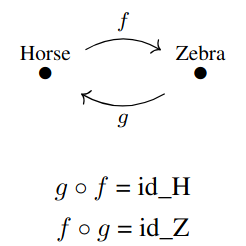
\includegraphics[width=0.2\textwidth]{figures/cyclegan_schema.png}     
    \caption[CycleGAN schema]{Schema for the cycleGAN architecture. (Image taken from \cite{gavranovic2019compositional}.)}
    \label{fig: cyclegan}
  \end{center}
\end{figure}


\begin{definition}[Model schema]
  The schema of a model represented by a multigraph $G$ is the freely generated category $\mathbf{Free}(G)$.
\end{definition}

The schema of a model does not contain any data nor does it do any computation, but it encodes the bare-bones structure of such model. If ${\sim}$ is the path congruence relation induced by the equations in $\mathcal{X}$, we can take the module $\mathbf{Free}(G)/{\sim}$ to impose the constraints represented by $\mathcal{X}$. Depending on the context, the word schema will refer either to $\mathbf{Free}(G)$ or to $\mathbf{Free}(G)/{\sim}$. We will see later that each equation in $\mathcal{X}$ can be associated with a specific loss function and these losses are used to teach models to abide by ${\sim}$.

Given a schema $\mathbf{Free}(G)$, we can choose an architecture for the model, that is, we can assign to each node a Euclidean space and to each morphism a parametric map. This procedure yields an untrained neural network.

\begin{definition}[Model architecture]
  Let $\mathrm{Free}(G)$ be a model schema. An architecture for such schema is a functor $\mathsf{Arch}: \mathrm{Free}(G) \to \mathbf{Para}_{\times}(\mathbf{Smooth})$ (see \textit{Def. \ref{def: para}} and see \textit{Ex. \ref{ex: smooth}}).
\end{definition}

The Euclidean spaces $\mathsf{Arch}$ maps objects to might be intuitively interpreted as the spaces the data will live in, but it is wiser to put data outside the $\mathbf{Para}$ machinery and in the simpler $\mathbf{Set}$ category, as this allows for better compartmentalisation. Thus, \cite{gavranovic2019compositional} also defines an embedding functor, which agrees with $\mathsf{Arch}$ on objects but exists independently of it.


\begin{definition}[Model embedding]
  Let $\mathrm{Free}(G)$ be a model schema and let $\mathsf{Arch}$ be a chosen architecture. An embedding for such schema is a functor $E: |\mathrm{Free}(G)| \to \mathbf{Set}$ which agrees with $\mathsf{Arch}$ on objects\footnote{The reason why the domain $E$ is the discretized schema $|\mathrm{Free}(G)|$ instead of the original schema $\mathrm{Free}(G)$ is clarified in \textit{Rem. \ref{rem: discretized}}.}.
\end{definition}

Now that we have a model, we must find a way to assign specific values to the parameters, so that the model can be optimized by gradient descent. Consider the function $\mathfrak{p}: (P,f) \mapsto P$, which takes the parameter space out of a parametric map in $\mathbf{Para}_{\times}(\mathbf{Smooth})$. We can use it to define the function 
\[\mathfrak{P}: \mathsf{Arch} \mapsto \prod_{f : \mathsf{Gen}_{\mathbf{Free}(G)}}\mathfrak{p}(\mathsf{Arch}(f)),\]
where $\mathsf{Gen}_{\mathbf{Free}(G)}$ is the set of generating morphisms of the free category on the multigraph $G$. The function $\mathfrak{P}$ takes and architecture and returns the parameter space. Given $\mathfrak{P}$, we can define the notion of parameter specification function.

\begin{definition}[Parameter specification function]
  Let $\mathrm{Free}(G)$ be a model schema and let $\mathsf{Arch}$ be a chosen architecture. A parameter specification function is a function $\mathsf{PSpec}$ which maps a pair $(\mathsf{Arch}, p)$ - comprised of an architecture $\mathsf{Arch}$ and some $p \in \mathfrak{P}(\mathsf{Arch})$ - to a functor $\mathsf{Model}_p: \mathbf{Free}(G) \to \mathbf{Smooth}$. The functor $\mathsf{Model}_p$ takes the model schema and returns its implementation according to $\mathsf{Arch}$, partially applying $p_f$ to each $\mathsf{Arch}(f)$, so that we obtain an actual smooth map. 
\end{definition}

The functor $\mathsf{Model}_p$ takes a schema and implements it replacing nodes with Euclidean spaces and arrows with appropriate smooth functions. Notice that, although we need to choose an architecture and specific values for its parameter in order to define $\mathsf{Model}_p$, the latter acts on the schema directly and does not pass through the architecture. See \textit{Fig. \ref{fig: layers}} for a srting diagram that depicts the relationship between $\mathsf{Arch}$ and $\mathsf{Model}_p$.

\begin{figure}[h]
  \begin{center}
    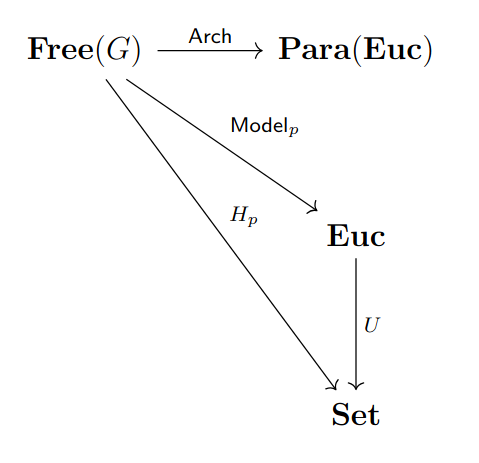
\includegraphics[width=0.35\textwidth]{figures/layers_of_abstraction.png}     
    \caption[CycleGAN schema]{Functors are used to link different layers of abstraction in the framework of \cite{gavranovic2019compositional}. (Image taken from \cite{gavranovic2019compositional}.)}
    \label{fig: layers}
  \end{center}
\end{figure}

Now, if we hope to train the model we have defined, we will need a dataset. \cite{gavranovic2019compositional} suggests that a dataset should be represented as a subfunctor of the model embedding functor.

\begin{definition}[Dataset]
  Let $E$ be a model embedding. Then, a dataset is a subfunctor $D_E: |\mathbf{Free}(G)| \to \mathbf{Set}$ which maps every object $A$ of the discretized free category $|\mathbf{Free}(G)|$ to a finite subset $D_E(A) \subseteq E(A)$.
\end{definition}

\begin{remark}
  \label{rem: discretized}
  The reason why \cite{gavranovic2019compositional} defines $E$ and $D_E$ on discretized categories is because it often happens in practical machine learning that the available data is not paired. In these cases, it would be meaningless to provide an action on morphisms because they would end up being incomplete maps.
\end{remark}

Given a node $A$ of $G$, we have associated to $A$ a Euclidean space $E(A)$ and a dataset $D_E(A)$. A dataset may be considered a collection of instances of something more specific than just vectors; for instance, if we have a finite dataset of pictures of horses, we are clearly interested in the concept of horse, that is in the set of all possible pictures of horses, which is much larger than our dataset but still much smaller than the vector space used to host such pictures. It makes thus sense to define another set $\mathfrak{C}(A)$ representing such concept: this set will satisfy the inclusion relations $D_E(A) \subseteq \mathfrak{C}(A) \subseteq E(A)$. Moreover, since concepts are assumed to be complete, we can extend $\mathcal{C}$ to a functor.

\begin{definition}[Concept functor]
  Given a schema $\mathbf{Free}(G)/{\sim}$, an embedding $E$ and a dataset $D_E$, a concept associated with this information is a functor $\mathfrak{C}: \mathbf{Free}(G)/{\sim} \to \mathbf{Set}$ such that, if $I: |\mathbf{Free}(G)| \to \mathbf{Free}(G)/{\sim}$ is the inclusion functor, $D_E \subseteq I \fatsemi \mathfrak{C} \subseteq E$.
\end{definition}

As \cite{gavranovic2019compositional} states, $\mathfrak{C}$ is an idealization, but it is a useful idealization as it represent the goal of the optimization process: given a dataset $D_E: |\mathbf{Free}(G)| \to \mathbf{Set}$, we wish to learn the concept functor $\mathfrak{C}: \mathbf{Free}(G)/{\sim} \to \mathbf{Set}$. More concretely, we want to train a model $\mathsf{Model}_p$ which is as close of an approximation of $\mathfrak{C}$ as possible\footnote{Notice that $\mathsf{Model}_p$ and $\mathfrak{C}$ have different domains and codomains. The difference of codomains is not an issue: we can just forget the differential structure of the codomain of $\mathsf{Model}_p$, which yields a functor $H_p$ with image in $\mathbf{Set}$ (see \textit{Fig. \ref{fig: layers}}). The difference of domains, on the other hand, is by design as $\mathsf{Model}_p$ can only approximate the constraints imposed by $\sim$. This is not an issue in practice as we are only interested in the performance of the image of the trained model $\mathsf{Model}_p$.}. Total achievement of such goal is clearly impossible as, even in the simplest of cases (such as linear regression on synthetic linearly generated data), finite arithmetics and the finite nature of the learning iteration prevent us from obtaining a perfect copy of the generating function.
Nevertheless, we will hopefully design an optimization process which makes the learning iteration converge towards the ideal goal.

Now that we know what the optimization goal is, we can define tasks. The task formalism brings together what has been defined in this section in an integrated fashion.

\begin{definition}[Task]
  Let $G$ be a directed multigraph, let ${\sim}$ be a congruence relation on $\mathbf{Free}(G)$ and let $D_E: |\mathbf{Free}(G)| \to \mathbf{Set}$ be a dataset. Then, we call the triple $(G,{\sim},D_E)$ a task.
\end{definition}

Once we are assigned a machine learning task $(G,{\sim},D_E)$, we have to choose an architecture, an embedding and a concept compatible with the given multigraph, equations and dataset. Then, we specify a random initial parameter with an appropriate parameter specification function. Now we can choose and optimizer, but we must be careful to choose an appropriate loss function. The loss function should incorporate both an architecture specific loss and a path equivalence loss. The former penalizes wrong predictions while the latter penalizes violations of the constraints embodied by ${\sim}$.

\begin{definition}[Path equivalence loss]
  Let $(G,{\sim},D_E)$ be a task. Let $\mathsf{Model}_p$ be an associated model. Then, if $f \sim g: A \to B$ in $G$, we define the path equivalence loss associated with $f$, $g$ and $\mathsf{Model}_p$ as 
  \[\mathcal{L}_{\sim}^{f,g} = \mathbb{E}_{a \sim D_E(A)}[\|\mathsf{Model}_p(f)(a) - \mathsf{Model}_p(g)(a)\|].\]  
\end{definition}

\begin{definition}[Total loss]
  Let $(G,{\sim},D_E)$ be a task. Let $\mathsf{Arch}$ be an associated architecture, let $\mathsf{Model}_p$ be an associated model, and let $\mathcal{L}'$ be an architecture specific loss. Suppose $\gamma$ is a non-negative hyperparameter. Then, we define the total loss associated with the task, the architecture, the model, and the hyperparameter as
  \begin{equation}
    \label{eq: sumoflosses}
    \mathcal{L} = \mathcal{L}' + \gamma\sum_{f \sim g}\mathcal{L}_{\sim}^{f,g}
  \end{equation}
\end{definition}

We can now proceed as usual, computing the loss on the dataset for a number of epochs and updating the parameter $p$ each time. Notice that $\mathcal{L}$ implicitly depends on $p$ because each $\mathcal{L}_{\sim}^{f,g}$ does.

It is important to notice that, while the learning iteration employed by \cite{gavranovic2019compositional} is nothing new, the functor approach is actually novel, in that the usual optimization process is used to explore a functor space instead of a simple morphism space. This point of view offers two main advantages: on one hand, it separates different layers of abstraction are separated providing much needed conceptual clarity; on the other hand, it offers an explicit treatment of constraints, which are often only described implicitly and hidden away in the architecture of the model or in the loss function. 

\subsection{Datasets influence the semantics of tasks}

\cite{gavranovic2019compositional} centers its investigation around the powerful cycleGAN architecture (\cite{zhu2017unpaired}), which is described using an appropriate task consisting of the cycleGAN schema (see \textit{Fig. \ref{fig: cyclegan}}), the cycle consistency equations, and a cycleGAN dataset, that is, a dataset with two sets $A$ and $B$ containing data which is essentially isomorphic, such as pictures of horses and zebras. This description is particularly insightful because it can be used to prove a very important point: the choice of dataset influences the semantics of the learned task in non-trivial ways. In other words, changing the dataset functor can result in semantically different tasks even if the same schema and equations are retained. 


The example shown in the paper is the \cite{gavranovic2019compositional}: combining the cycleGAN schema with the cycleGAN equations and a cycleGAN dataset yields a task whose semantics can be described as \textit{learn maps that turn horses into zebras and vice versa}. Now replace the cycleGAN dataset with a new dataset consisting of two sets $A$ and $B$, where $A$ contains pictures depicting two elements $X$ and $Y$ together, and $B$ contains separate images of $X$ and $Y$. The resulting task has very different semantics: \textit{learn how to separate $X$ from $Y$}. For instance, \cite{gavranovic2019compositional} shows how to use the CelebA dataset to train a neural network able to remove glasses from pictures of faces, or even insert them.


This example is especially relevant to the present discussion because it shows how important the categorical structure of $\mathbf{Set}$ can be to machine learning. We can interpret pairs \textit{(face, glasses)} as elements of the Cartesian product of the set of faces and the set of glasses. On the other hand, the set of pictures of faces with glasses can instead be considered another categorical product of the aforementioned sets. Since categorical products are unique, we know that there must be a unique isomorphism between the two products. Then, one interpretation of the task becomes: \textit{find the canonical isomorphism}. \cite{gavranovic2019compositional} labels this task as the product task and shows empirical evidence of the validity of the approach.





\section{Categorical representation learning}



We now discuss frameworks where the categorical structure of data is not only used to integrate data distributed among different sets (as in \cite{gavranovic2019compositional}) but also to model relationships within the data. Preserving and exploiting this structure functorially can lead to marked improvements in effectiveness and efficiency of the models in question  because the structure of data is often closely linked with its semantics (see e.g. \cite{sheshmani2021categorical}), especially in the field of natural language processing, or NLP (see e.g. \cite{coecke2010mathematical}, \cite{lewis2019compositionality}). 


The field of \textit{categorical representation learning} (\cite{coecke2010mathematical}, \cite{lewis2019compositionality}, \cite{sheshmani2021categorical}) aims to learn vectorial representations of data endowed with a categorical structure mirroring the one of the original data, so that models tranined on these representations can use the structure efficiently. This is often a symbolic-to-vectorial transformation, which poses conceptual and computational challenges (see e.g. \cite{coecke2010mathematical}). We will examine two examples of categorical representation learning: the approach of \cite{sheshmani2021categorical}, which uses the obtained representations to carry out (partially) unsupervised translation, and the approaches of \cite{coecke2010mathematical} and \cite{lewis2019compositionality}, which develop a compositional distributional model of meaning for NLP.




\subsection{Unsupervised functorial translation}


We now illustrate the approach of \cite{sheshmani2021categorical} showing how it is applied to the same example described in the original paper: unsupervised translation of the names of chemical elements from English to Chinese. The authors are tasked with converting between two identical chemical compound datasets, one labeled in English and the other in Chinese. Both datasets can be given a categorical structure by considering elements as objects and chemical bonds as morphisms. Suppose $\mathcal{C}$ and $\mathcal{D}$ are the resulting categories. The authors of \cite{sheshmani2021categorical} leverage the share structure by training a model to learn a translation functor $\mathcal{F}: \mathcal{C} \to \mathcal{D}$. To this aim, they then functorially embed these categories into the vector space category defined below, which will contain representations as objects.


\begin{definition}[Vector space category]
  \label{def: vecspacecat}
  Let $n \in \mathbb{N}$. Let $\mathcal{R}$ be the category whose objects are the vectors in $\mathbb{R}^n$ and such that, for all $u,v :\mathcal{R}$, 
  \[\mathcal{R}(u, v) = \{M \in \mathbb{R}^{n \times n} \text{ s.t. } v = Mu\}.\]
  Composition is ordinary matrix multiplication and the identity on $v$ is $\mathrm{id}_v = \frac{vv^T}{|v|^2}$.
\end{definition}



The embedding of $\mathcal{C}$ into $\mathcal{R}$ is   $\mathcal{C} \to \mathcal{R}$ functor which maps each object $a$ to a vector $v_a$ and each morphism $f$ to a matrix $M_f$. The actual mapping can be learned with a neural network consisting of two separate embedding layers: one mapping objects to vectors and one mapping relations to matrices. The authors of \cite{sheshmani2021categorical} train the embedding layers using co-occurrence statistics and negative sampling to make sure that the embedded morphisms actually represent the same relations as the original morphisms. Here, the authors of \cite{sheshmani2021categorical} take on a distributional point of view, positing that co-occurrence must encode such relations. In the authors' words, \lq  co-occurrence does not happen for no reason\rq. The training strategy used in the paper is the following: given two embedded words $a$ and $b$, model the probability of co-occurrence as $P(a \to b) = \mathsf{sigmoid}(z(a \to b))$, where the logit $z(a \to b)$ is defined as
\[z(a \to b) = F\left(\bigoplus_f v_a^TM_fv_b \right).\]
Here, $F$ is non-linear and $\oplus_f$ represents concatenation (or more sophisticated forms of aggregation) over all morphisms in $\mathcal{C}$. Taking on a probabilistic perspective allows us to represent non-strict relations, which is often necessary in machine learning. From this point of view, the likelihood of $f: a \to b$ is proportional to the degree of alignment between $v_b$ and $M_fv_a$ are closely aligned. The latter can be computed as $v_a^TM_fv_b$, and the non-linearity $F$ reads out these measurements into a single value. Now, the actual co-occurrence probability $p(a,b)$ of two objects $a,b : \mathcal{C}$ can be approximated directly from the dataset. Given a negative sampling distribution $p_N$ on objects unrelated to $a$, we can implement the negative sampling objective
\[\mathcal{L} = \mathbb{E}_{(a,b) \sim p(a,b)}\left(\log P(a \to b) + \mathbb{E}_{b' \sim p(b')}\log (1-P(a \to b'))\right).\]
The embedding network can then be trained by maximizing this objective function. The embedding of $\mathcal{D}$ into $\mathcal{R}$ can be defined and trained in the same way.

\begin{remark}
  Strictly speaking, morphisms in category should have a specific domain and a specific codomain but, in the case of the vector space category of \textit{Def. \ref{def: vecspacecat}}, a single matrix $M$ can be in many hom-sets of $\mathcal{R}$. This is mirrored by $\mathcal{C}$ and $\mathcal{D}$, where morphisms correspond to classes of chemical bond and the same morphism can link different objects. From this point of view, morphisms in $\mathcal{R}$, in $\mathcal{C}$, and in $\mathcal{D}$ behave more similarly to relations on sets than to morphisms in categories.  Although this line of thinking does not strictly adhere to the definition of category, it helps our intuition and greatly reduces the size of the model by limiting the number of parameters that need to be learned. We will see a possible formal solution to this problem later on in this section, when we discuss the approach of \cite{coecke2010mathematical} and \cite{lewis2019compositionality}.
\end{remark}

The procedure described above can be been applied to both $\mathcal{C}$ and $\mathcal{D}$ to obtain meaningful vectorial representations of both datasets. An English to Chinese translation functor $\mathcal{F}: \mathcal{C} \to \mathcal{D}$ can be similarly embedded as a $\mathcal{R} \to \mathcal{R}$ functor by precomposition with the $\mathcal{C} \to \mathcal{R}$ embedding and postcomposition with the inverse of the $\mathcal{D} \to \mathcal{R}$ embedding. Such functor must equate chemical bonds of the same kind, for example, if $f$ is a covalent bond so is $\mathcal{F}(f)$. It is argued in \cite{sheshmani2021categorical} that this functor can be represented by a matrix $V_\mathcal{F}$ so that $v_{\mathcal{F}(a)} =  V_\mathcal{F}v_a$ and $M_{\mathcal{F}(f)} = V_\mathcal{F}M_f$. This representation is only meaningful if (i) $V_{\mathcal{F}}M_f = M_{\mathcal{F}}V_{\mathcal{F}}$ for all $f$, (ii) $V_{\mathcal{F}}M_{\mathrm{id}_a} = M_{\mathrm{id}_{\mathcal{F}(a)}}$ for all $a$, and (iii) $V_{\mathcal{F}}M_{f \circ g} = V_{\mathcal{F}}M_fV_{\mathcal{F}}M_g$ for all $f,g$. This is not true for all choices of  $V_\mathcal{F}$ but, if we choose every $v_a$ to be a unit vector, and if we constrain $V_{\mathcal{F}}$ to be orthogonal, (ii) and (iii) are trivially satisfied. Requirement (i), on the other hand, can be learned by minimizing the following structure loss:
\[\mathcal{L}_{\mathrm{struc}} = \sum_{f}\|V_{\mathcal{F}}M_f - M_{\mathcal{F}(f)}V_{\mathcal{F}}\|^2.\]
As the authors of \cite{sheshmani2021categorical} remark, this loss is universal, in the sense that it does not depend on any specific object, but acts on the morphisms themselves. While this approach is very elegant and does indeed return a functor, it might not produce the functor we expect because $V_{\mathcal{F}}$ is not unique if the $M_f$ happen to be singular. Thus, it is better to integrate the structure loss with a second alignment loss that introduces some supervision to the unsupervised translation task. For instance, if the value of $\mathcal{F}(a)$ is known for a set $A$ for objects, we can define
\[\mathcal{L}_{\mathrm{align}} = \sum_{a \in A}\|V_{\mathcal{F}}v_a - v_{\mathcal{F}(a)}\|.\]
Then, the total loss can be written as a weighted sum 
\begin{equation}
  \label{eq: sumoflosses2}
  \mathcal{L} = \mathcal{L}_{\mathrm{align}} + \lambda \mathcal{L}_{\mathrm{struct}},
\end{equation}
where $\lambda$ is a hyperparameter that regulates the relative importance of the two losses.

\begin{remark}
  It is interesting to compare the total loss in \textit{Eq. \ref{eq: sumoflosses2}} to the one in \textit{Eq. \ref{eq: sumoflosses}}. In both cases, the total loss is obtained as a linear combination of a model specific loss and a second more abstract loss. Both abstract losses enforce equality between morphisms but the abstract loss in \textit{Eq. \ref{eq: sumoflosses2}} does not enforce functoriality because $\mathsf{Model}_p$ is already a functor by definition in the framework of \cite{gavranovic2019compositional}. This highlights the main difference between the approach of \cite{gavranovic2019compositional} and the approach of \cite{sheshmani2021categorical}: the latter requires functoriality to be learned from structure of data, while the former takes functoriality as a given.
\end{remark}


According to \cite{sheshmani2021categorical}, the categorical approach described above can also be strengthened by endowing the categories $\mathcal{C}$, $\mathcal{D}$, and $\mathcal{R}$ with monomial products that make combining objects into higher-level structures possible. In particular, the monomial structure $\otimes'$ of $\mathcal{R}$ can be given as
\begin{align*}
  v_a \otimes' v_b &= \Theta(v_a \otimes v_b),\\
  M_f \otimes' M_f &= \Theta(M_f \otimes M_g),\\
\end{align*}
where $\otimes$ is the Kronecker tensor product and $\Theta$ is a learned operator that sends the products back into the original spaces. This monomial structure can then be used to mine categorical structure on multiple levels: for instance, in the running example of unsupervised translation of chemicals, it can be used to derive vectorial representations for functional groups or even whole compounds. If the data has a non-obvious high-level structure, \cite{sheshmani2021categorical} suggests a bootstrap approach where different possible links are randomly tested and the stronger ones are selected.


It is shown in \cite{sheshmani2021categorical} that the categorical representation learning framework described in the paper and the associated functor learning architecture for unsupervised translation can be successfully implemented. Benchmark tests against traditional sequence-to-sequence models show that the functorial paradigm leads to marked improvements in efficiency of learning. In particular, the authors compare a GRU cell model of similar performance as the functorial model described in the paper, noting that the former needs 17 times more parameters than the latter to learn to translate element names with a similar accuracy. The authors also compare their approach with the multi-head attention approach first introduced by \cite{vaswani2017attention}, arguing that their categorical approach is an improvement over multi-head attention as the matrices $M_f$ are essentially equivalent to the products $Q_f^TK_f$, where $Q_f$ is the query matrix associated to $f$ and $K_f$ is the key matrix associated to $f$. Keeping $M_f$ united emphasizes the important role of functoriality and provides intuition concerning the nature of the vectorial representations of objects: in fact, it makes sense to interpret each $M_f$ as a metric that distorts the space $\mathbb{R}^n$ and makes two vectors $v_a$ and $v_b$ closer if and only if there is a high likelihood that $a \stackrel{f}{\longrightarrow} b$.



\subsection{Compositional distributional model for NLP}

There are two general approaches to natural language processing (NLP): the \textit{compositional} approach and the \textit{contextual} approach. The former aims to exploit the symbolic structure of grammar to understand text, while the latter posits that many aspects of text can be understood from distributional properties of the words (\cite{amigo2022information}). While compositionality has been very popular with theoreticians due to its elegance and its abstract structure, contextuality has been successfully applied by practitioners, yielding remarkably effective NLP models that learn the meaning of words and utterances by embedding them in vector spaces. These embeddings are mostly based on contextual information. The fact that both compositionality and contextuality are successful in their domains hints that the two approaches should be seen as complementary and that it would be auspicable to integrate them both in a single \textit{compositional distributional framework}\footnote{Cognitive science faces a similar challenge in integrating the competing connectionists and symbolic models of the human mind. This is the central theme of \cite{smolensky2006harmonic}, whose approach inspired \cite{clark2007combining} (discussed in this section). The important role of language in cognition suggests that advances in the development of a compositional distributional model of language may yield advances in cognitive science and vice versa.} (see e.g. \cite{amigo2022information}, \cite{maruyama2019compositionality}). 


There have been numerous attempts to develop such a framework in the last few decades. For instance, \cite{clark2007combining} proposes to represent both text and the structural roles of its constituents as vectors, which can then be combines using sums and tensor products. We will focus on the approach of \cite{coecke2010mathematical}, whose authors take inspiration from the ideas in \cite{clark2007combining} and propose a framework that uses the language of compact closed categories to unite symbolic grammar rules with concrete representation vectors. Grammar is represented as a pregroup category, whereas vectorial representations are learned on vector spaces which are then organized within $\mathbf{FVect}$, the category of finite dimensional real vector spaces. We start by defining pregroup categories\footnote{We work under the same assumption as \cite{coecke2010mathematical}, namely, that each vector space in $\mathbf{FVect}$ is endowed with a scalar product $\langle-,-\rangle$.}.

\begin{definition}[Pregroup]
  A pregroup is a monoidal poset category $P$ where each object $a$ has a left adjoint $a^l$ and a right adjoint $a^r$. The adjoints must be such that the following are true:
  \begin{align*}
    a^la \leq &1 \leq aa^l,\\
    aa^r \leq &1 \leq a^ra,
  \end{align*}
  where $1$ is the monoidal unit of $P$.
\end{definition}

The use of pregroups to model grammatical structures dates back to \cite{lambek1999type}. The key idea is that we can define a grammar category as the free pregroup $P$ generated by an initial set of basic grammatical roles. Then, we can represent various parts of speech using basic objects, their adjoints, and their monomial products. The poset structure of the pregroup serves as a system of reduction rules which can be used to prove if a sentence is grammatical. Consider the following example (taken from \cite{lewis2019compositionality}).


\begin{example}
  Suppose $n$ represents the role of a noun and $s$ represents the role of a sentence. Then, an English transitive verb can be represented by the product $n^rsn^l$ in the pregroup $P$ generated by $s$ and $n$. Thus, the grammatical structure of the sentence \dblquote{Dragons breathe fire.} is
  \begin{equation}\
    \label{eq: grammreduction}
    n(n^rsn^l)n = nn^rsn^ln = (nn^r)s(n^ln) \leq 1s1 \leq s.
  \end{equation}
  The pregroup axioms show that the structure of  \dblquote{Dragons breathe fire.} can be reduced to the sentence type $s$. This is proof that the sentence is grammatical. More complex patter can be modeled by adding more grammatical types or by combining types in other ways. These kinds of computations have a nice representation in the form of string diagrams such as the ones of \textit{Fig. \ref{fig: pregroup}}.
\end{example}

\begin{figure}[h]
  \begin{center}
    \begin{subfigure}{0.32\textwidth}
      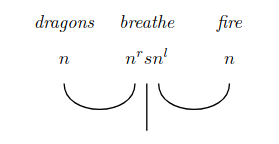
\includegraphics[width=\textwidth]{figures/pregroup1.png}
      \caption{}
    \end{subfigure}
    \begin{subfigure}{0.47\textwidth}
      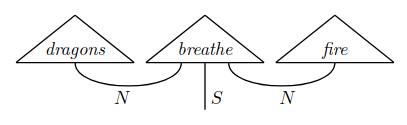
\includegraphics[width=\textwidth]{figures/pregroup2.png}
      \caption{}
    \end{subfigure}         
    \caption[Pregroup representation of grammar]{Two string diagram representations of the grammatical structure of the sentence \dblquote{Dragons breathe fire.} (Images taken from \cite{lewis2019compositionality}.)}
    \label{fig: pregroup}
  \end{center}
\end{figure}

The pregroup grammar framework is useful to analyze the basic structure of language but gives no access to the actual meaning of words and sentences. The compositional distributional model of \cite{coecke2010mathematical} solves this problem by building a functor $\Phi: P \to  \mathbf{FVect}$. Given a certain pregroup grammar category $P$, for every grammatical type $x: \mathcal{P}$, we can associate a vector space $X:\mathbf{FVect}$ containing vectorial representations of utterances of type $x$. $\Phi$ can be defined so that it preserves the pregroup structure of $P$ thanks to the following proposition (\cite{coecke2010mathematical}).

\begin{proposition}
  Consider the category $\mathbf{FVect}$ of finite-dimensional real vector spaces. Suppose $\otimes$ is the tensor product of vector spaces. Then, $(\mathbf{FVect}, \mathbb{R}, \otimes)$ is a monoidal category.  
  For all $V: \mathbf{FVect}$, define $V^l = V^r = V$ and consider the (co)unit linear maps:
  \begin{align*}
    \eta_V^l = \eta_V^r: \mathbb{R} \to V \otimes V, \,\,\, &1 \mapsto \sum_i e_1 \otimes e_1,\\
    \epsilon_V^l = \epsilon_V^r: V \otimes V \to \mathbb{R}, \,\,\, &\sum_{i,j} c_{ij} e_i \otimes e_j \mapsto \sum_{i,j} c_{ij} \langle e_i, e_j \rangle,
  \end{align*}
  where $e_1, \dots, e_n$ is a basis for $V$. Then, $(\mathbf{FVect}, \mathbb{R}, \otimes, (-)^l, (-)^r, \eta^l, \eta^r, \epsilon^l, \epsilon^r)$ is a compact closed monoidal category.
\end{proposition}

Now, pregroups have a trivial compact-closed structure as well. Thus, the functor $\Phi$ can be defined so that it preserves the shared compact-closed structure just by mapping the poset relatioins of $P$ to the appropriate linear maps of $\mathbf{FVect}$. In practice, $\Phi$ can be used to take a formal reduction in $P$ and implement it in $\mathbf{FVect}$ as a series of operations on vectorial representations. The goal of this process is to take vectorial representations of single words in a sentence and obtain the vectorial representation of the meaning of the sentence. The compositional distributional model is thus compositional because it is build around the compositional structure of grammar and distributional because it allows us to encode distributional information in vectorial representations of words and sentences.

\begin{example}
  The reduction of \textit{Eq. \ref{eq: grammreduction}} can be seen as a morphism $nn^rsn^ln \to s$. The image of this morphism through $\Phi$ is a linear map 
  $N \otimes N \otimes S \otimes N \otimes N \to S.$
\end{example}

\begin{remark}
  Differently from \cite{sheshmani2021categorical}, \cite{coecke2010mathematical} does not prescribe a specific method for learning the representations of individual words (some possible strategies are listed in the original paper), but specifies a strategy to combine existing representations to generate representations of more complex utterances up to the level of whole sentences. It is interesting to notice that both papers suggest using tensor products in order to combine representations of lower-level structures into representations of higher-level structures.
\end{remark}


String diagrams such as the ones in \textit{Fig. \ref{fig: pregroup}} can be written down as binary trees thanks to the associativity of the monomial product of $P$ and the associativity of the tensor product of $\mathbf{FVect}$. 
\cite{lewis2019compositionality} proposes to exploit this fact and augment the compositional distributional model of \cite{coecke2010mathematical} by implementing the (co)unit maps of $\mathbf{FVect}$ as one or more recursive neural network (TreeRNN) cells. The paper argues that the use of TreeRNN cells should make the model easier to train and more robust. To our knowledge, such proposal has not yet been implemented, although the use of TreeRNNs in NLP has already been applied in practice (see e.g. \cite{ahmed2019improving}).





\section{Equivariant neural networks as functors}

\begin{warning}
  We warn the reader that the paper \cite{chytas2024poolingimagedatasetsmultiple}, whose contents are discussed in this section, has been \textit{withdrawn by the authors} citing issues with the references. We decided against omitting the paper from this thesis because we think its research direction is intriguing and potentially highly valuable. Hopefully, future research will soon clarify the epistemological status of the ideas hereby discussed.
\end{warning}

\cite{chytas2024poolingimagedatasetsmultiple} presents a categorical framework that describes neural network layers as functors and uses their functorial nature to impose invariance and equivariance constraints. In particular, equivariance constraints are used to effectively transport the unary operators from the dataset into a latent embedding layer. It is shown that this enables the creation of models that account for shifts and imbalance in covariates when being trained on pooled medical image datasets. In this section, we describe the framework of \cite{chytas2024poolingimagedatasetsmultiple} and we draw a short comparison with the work of \cite{pfrommer2024transport}, which also deals with the transport of algebraic structure into embedding layers.


\subsection{An equivariant classifier to diagnose Alzheimer's disease}

The authors of \cite{chytas2024poolingimagedatasetsmultiple} consider a data category $\mathcal{S}$ whose objects $s$ are data points and whose morphisms $f: s_1 \to s_2$ represent differences in covariates. An example considered in the paper is the following: suppose the objects $s$ are comprised of brain scans and associated information concerning patient age and other covariates. The goal is to develop a model trained to diagnose Alzheimer's disease from the scans. An example of morphism in such data category is $f_x: s_1 \to s_2$, which indicates a difference of $x$ years in age\footnote{Notice that this kind of operator clearly possesses an algebraic structure as $f_x \fatsemi f_y = f_{x+y}$.}: $s_2.\mathrm{age} = s_1.\mathrm{age} + x$. Since we are dealing with a classification task, the dataset here has labels. It is important not to include the labels in the data category, else any classifier model would just read such labels instead of learning to predict them. Use the notation $\mathbf{y}_s$ to represent the label associated to $s$. Since the dataset has labels while the data category must not have them, we feel justified in using the phrase data category in place of the phrase dataset category employed above.

Now, if we consider another category $\mathcal{T}$, we can use a functor $F: \mathcal{S} \to \mathcal{T}$ to project $\mathcal{S}$ onto $\mathcal{T}$. Learning such functor instead of a simple map between objects is advantageous because the functoriality axioms imply that $F$ automatically satisfies equivariance constraints: if $g: s_1 \to s_2$,
\begin{equation}
  \label{eq: categorical_equivariance}
  F(g): F(s_1) \to F(s_2).
\end{equation}
Invariance with respect to $g$ is not much harder to define: it suffices to impose $F(s_1) = F(s_2)$ and $F(g) = \mathrm{id}_{F(s_1)}$.

\begin{remark}
  \textit{Eq. \ref{eq: categorical_equivariance}} is a categorical generalization of the more usual group-theoretical notion of invariance, as defined in \textit{Def. \ref{def: equivariance}}. To be precise, \textit{Def. \ref{def: equivariance}} is equivalent to \textit{Eq. \ref{eq: categorical_equivariance}} if $\mathcal{S}$, $\mathcal{T}$ are Borel spaces and $g$, $F(g)$ are group actions, as highlighted in \cite{chytas2024poolingimagedatasetsmultiple}.
\end{remark}


The authors of \cite{chytas2024poolingimagedatasetsmultiple} solve the Alzheimer's disease diagnosis task using a classifier that actively exploits the equivariant nature of functors. The proposed architecture consists of two modules: an invertible functor $F: \mathcal{S} \to \mathcal{T}$ that embeds the data into a latent space, and a functor $C: \mathcal{T} \to \mathbf{Free}(\mathbb{N})$ that does the actual classification (see \textit{Fig. \ref{fig: classifier}} for a diagrammatic representation). Here, $\mathcal{T}$ acts as a latent space and the equivariance of $F$ forces the representations in $\mathcal{T}$ to be robust with respect to covariate shifts and imbalances, so that the actual classification operated by $\mathcal{C}$ can be more effective at diagnosing the disease. The whole model can be compactly represented as $F \fatsemi C: \mathcal{S} \to \mathbf{Free}(\mathbb{N})$. Although the inverse of $F$ does not appear in the formula, its existence is needed to ensure that the latent space accurately represents the data.

\begin{figure}[h]
  \begin{center}
    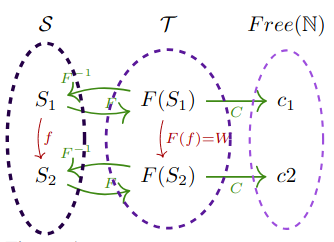
\includegraphics[width=0.35\textwidth]{figures/classifier.png}     
    \caption[Classifier]{Classifier model proposed by \cite{chytas2024poolingimagedatasetsmultiple} (Image taken from \cite{chytas2024poolingimagedatasetsmultiple}.)}
    \label{fig: classifier}
  \end{center}
\end{figure}



The classifier described above is implemented using similar tools as the ones employed by \cite{sheshmani2021categorical}. The latent space $\mathcal{T}$ can be defined as a vector space category as in \textit{Def. \ref{def: vecspacecat}}. The functor $F$ is realized as the encoder of an appropriate autoencoder, and the decoder portion of this autoencoder acts as the inverse $F^{-1}$. The maps $f: \mathcal{S}(s_1,s_2)$ can be embedded as matrices as described in the previous section. In particular, \cite{chytas2024poolingimagedatasetsmultiple}  suggests using orthogonal matrices $F(f) = W_f$ so that the resulting transformations can be efficiently inverted.
Finally, $C$ can be implemented as a MLP classifier.

Now that the architecture has been specifies in terms of neural networks, the resulting model can be trained using gradient descent and a linear combination of three separate losses: $\mathcal{L} = \gamma_1\mathcal{L}_r + \gamma_2\mathcal{L}_p + \gamma_3\mathcal{L}_s$, where $\gamma_1$, $\gamma_2$, and $\gamma_3$ are hyperparameters. Here, $\mathcal{L}_r$ is a reconstruction loss, which makes sure that $F$ is invertible and that its inverse accurately reconstructs the original data; $\mathcal{L}_p$ is a prediction loss, which makes sure that $F \fatsemi C$ accurately predicts the labels of the data; $\mathcal{L}_s$ a structure loss, which makes sure that $F$ acts as a functor and not just a map. In formulas,
\[\mathcal{L}_r = \sum_{s : \mathcal{S}}\|s-(F^{-1} \circ F)(s)\|^2_2,\]
\[\mathcal{L}_p = \sum_{s : \mathcal{S}}\mathsf{crossentropy}(\mathbf{y}_s,(C \circ F)(s)),\]
\[\mathcal{L}_s = \sum_{\begin{smallmatrix}s_1, s_2 : \mathcal{S} \\ f: s_1 \to s_2 \end{smallmatrix}}\|W_fF(s_1)-F(s_2)\|^2_2.\]

\begin{remark}
  Notice that the amount of equivariance constraints imposed can vary with no substantial changes to the proposed architecture: it suffices to add or remove terms from $\mathcal{L}_s$. This is in stark contrast with approaches such as \cite{lokhande2022equivariance}, where handling multiple covariates requires a complicate multi-stage model. 
\end{remark}

The authors of \cite{chytas2024poolingimagedatasetsmultiple} test the validity of the proposed approach with two interesting experiments: a proof of concept trained on the MNIST dataset, and a working classifier trained on the ADNI brain imaging dataset. The proposed MNIST model implements equivariance with respect to increments, rotations, and zooming. It is shown in the paper that representing the associated morphisms with orthogonal matrices allows such morphisms to be inverted and combined in the latent space. A subsequent application of $F^{-1}$ shows the results of the aforementioned manipulation in human-understandable form. Such results are indeed very promising: the authors are able to combine rotations and scaling successfully, even though the network was only trained to apply them separately (see \textit{Fig. \ref{fig: rotationsscaling}}) for an example. The ADNI classifier model also shows promising results which are on par with state-of-the-art models that do not use categorical tools. The comparison takes place according to accuracy of prediction, maximum mean discrepancy, and adversarial validation.

\begin{figure}[h]
  \begin{center}
    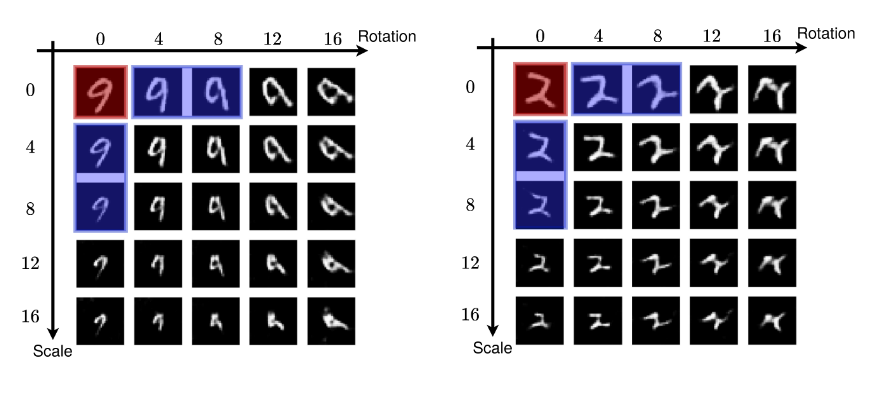
\includegraphics[width=0.7\textwidth]{figures/rotations_and_scaling.png}     
    \caption[Classifier]{The authors of \cite{chytas2024poolingimagedatasetsmultiple} applied rotations and scaling on MNIST images using the operators learned in the latent space. Despite being learned separately, the two transformations were successfully combined. (Image taken from \cite{chytas2024poolingimagedatasetsmultiple}.)}
    \label{fig: rotationsscaling}
  \end{center}
\end{figure}

\subsection{Transporting algebraic structure into embedding spaces}

Although stated in terms of equivariance conditions, the work of \cite{chytas2024poolingimagedatasetsmultiple} can be seen from an algebraic point of view as a framework that allows to transport unary operators from a space of data to an embedding space. This line of thinking has also been explored by \cite{pfrommer2024transport}. While \cite{pfrommer2024transport} deos not use category theory, the authors themselves state that their approach could be easily categorified using the language of categorical algebras (see \textit{Def. \ref{def: endalg}}). The main innovation of \cite{pfrommer2024transport} is the use of \textit{mirrored algebras} to fill the gaps between original data and the embeddings.


Consider a pre-trained autoencoder consisting of an encoder $E: \mathcal{S} \to \mathcal{L}$ and a decoder $D: \mathcal{L} \to \mathcal{S}$, where $\mathcal{S}$ is a data space endowed with an algebraic structure, such as a monomial product $\bullet^{\mathcal{S}}$, and where $\mathcal{L}=\mathbb{R}^n$ is a latent space. Suppose we want to transport this algebraic structure to $\mathbb{R}^n$ through $E$, that is, we want to find a monomial product $\bullet^{\mathcal{L}}$ over $\mathcal{L}$ so that $E$ acts as a $(\mathcal{S},\bullet^{\mathcal{S}}) \to (\mathcal{L},\bullet^{\mathcal{L}})$ homomorphism. While finding a product $\ast$ that makes $(\mathcal{S},\bullet^{\mathcal{S}})$ and $(\mathcal{L},\bullet^{\mathcal{L}})$ homomorphic might be easy, there is no guarantee that $E$ is an actual homomorphism with respect to this choice of algebraic structure. \cite{chytas2024poolingimagedatasetsmultiple} solves this problem for unary operators by learning appropriate orthogonal matrices, but it is not clear how this approach could be scaled to operators with arities greater than $1$.  \cite{pfrommer2024transport} suggests an alternative approach consisting in learning a bijection $\phi$ between the latent space and a copy $\mathcal{M} = \mathbb{R}^n$ of this space. Endow $\mathcal{M} = \mathbb{R}^n$ with a product $\bullet^{\mathcal{M}}$ which enjoyes similar properties as $\bullet^{\mathcal{S}}$ (see \textit{Fig. \ref{fig: algtranspor}}). We will say that $(\mathcal{M},\bullet^{\mathcal{M}})$ is the mirrored algebra of $(\mathcal{S},\bullet^{\mathcal{S}})$. Now train $\phi$ so that $E$ is $(\mathcal{S},\bullet^{\mathcal{S}}) \to (\mathcal{L},\bullet^{\mathcal{L}})$ homomorphism, where $\bullet^{\mathcal{L}}$ is defined by
\[l_1 \bullet^{\mathcal{L}} l_2 = \phi^{-1}(\phi(l_1) \bullet^{\mathcal{M}} \phi(l_2)).\]

\begin{figure}[h]
  \begin{center}
    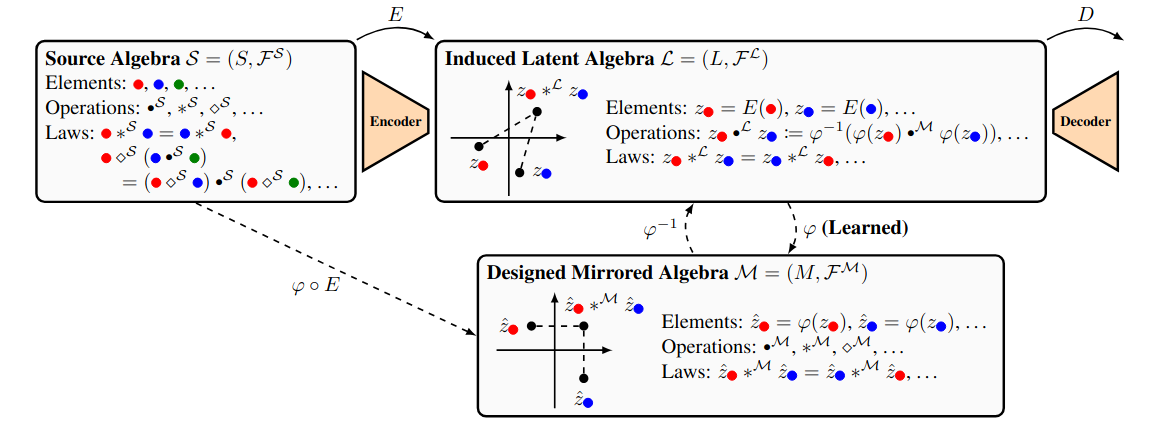
\includegraphics[width=1\textwidth]{figures/transport_of_algebraic_structure.png}     
    \caption[Transport of algebraic structure]{Method proposed by \cite{pfrommer2024transport} to transport algebraic structure. (Image taken from \cite{pfrommer2024transport}.)}
    \label{fig: algtransport}
  \end{center}
\end{figure}

As stated in \cite{pfrommer2024transport}, the bijection $\phi$ can be implemented as an invertible neural network and can be trained using a loss in the form
\[\mathcal{L} = \frac{1}{N}\sum_{i=1}^N d(D(p_i^{\mathcal{L}}(E(s_1),\dots,E(s_{n_i}))),p_i^{\mathcal{S}}(s_1, \dots, s_{n_i}))\]
where the $p_i^{\mathcal{S}}$ are algebraic expressions sampled from the set of expressions over $(\mathcal{S},\bullet^{\mathcal{S}})$, the $s_j$ are sampled from $\mathcal{S}$, $p_i^{\mathcal{L}}(t_1,\dots,t_{n_i})$ is defined as $\phi^{-1}(p_i^{\mathcal{M}}(\phi(t_1),\dots,\phi(t_{n_i})))$, $p_i^{\mathcal{M}}$ is the translation of $p_i^{\mathcal{S}}$ in terms of the algebraic structure of $(\mathcal{M},\bullet^{\mathcal{M}})$, and $d$ is an appropriate distance function.


We only presented a sketch of the work in \cite{pfrommer2024transport}: the original paper presents the framework in terms of any general algebraic structure, deals with laws that regulate the interaction of different operations, proves theoretical guarantees, and explores limitations of the proposed approach. It is shown in the paper that it is not always possible to find a mirrored algebra whose operations satisfy the same laws of the source algebra, which means that it is not always possible to transport this algebraic structure in its entirely. Nevertheless, the authors carry out experiments that prove that there are tangible advantages even in transporting a subset of the algebraic laws. The experiments support the following conjecture: \dblquote{learned latent space operations will achieve higher performance if they are constructed to satisfy the laws of the underlying source algebra} (\cite{pfrommer2024transport}). 





\clearpage{\pagestyle{empty}\cleardoublepage}
























































































%%%%%%%%%%%%%%%%%%%%%%%%%%%%%% CONCLUSIONS %%%%%%%%%%%%%%%%%%%%%%%%%%%%%%%%%%%

\chapter*{Conclusions}
\rhead[\fancyplain{}{\bfseries
Conclusions}]{\fancyplain{}{\bfseries\thepage}}
\lhead[\fancyplain{}{\bfseries\thepage}]{\fancyplain{}{\bfseries Conclusions}}
\addcontentsline{toc}{chapter}{Conclusions} 




\clearpage{\pagestyle{empty}\cleardoublepage}





%%%%%%%%%%%%%%%%%%%%%%%%%%%%%%%%%%%%% BIBLIOGRAPHY %%%%%%%%%%%%%%%%%%%%%%%%%%%%%%

\bibliographystyle{alpha}
%{\footnotesize \bibliography{references}}
{\bibliography{references}}
\rhead[\fancyplain{}{\bfseries \:Bibliography}]{\fancyplain{}{\bfseries\thepage}} 
\addcontentsline{toc}{chapter}{Bibliography}



\clearpage{\pagestyle{empty}\cleardoublepage}




%%%%%%%%%%%%%%%%%%%%%%%%%%%%%%%%%%%%%%% ACKNOWLEDGEMENTS %%%%%%%%%%%%%%%%%%%%%%%%%%%

\chapter*{Acknowledgements}

\thispagestyle{empty}

I wish to acknowledge the essential role my advisor Professor F. Zanasi has had in guiding me through the process of writing this thesis. He introduced me to applied category theory, to machine learning, and to the world of academic research, and I will be forever grateful for it. I also wish to thank my family and my friends, who supported me throughout this journey, and without whom all of this would not have been possible. To all of you, my most sincere gratitude.



\end{document}
